\documentclass[english,10pt,a4paper]{book}
\usepackage[T1]{fontenc}
\usepackage[left=3cm, right=3cm, top=2cm, bottom=2cm]{geometry}
\usepackage[backend=biber, style=apa]{biblatex} % Example with APA style
\addbibresource{references.bib} % Your bibliography file
\usepackage{graphicx}
\usepackage{float}
\usepackage{mathtools}
\usepackage{amssymb}
\usepackage{amsthm}
\usepackage{babel}
\usepackage{hyperref}
\usepackage{listings} % Package for code formatting
\usepackage{xcolor}    % Colors for syntax highlighting
\usepackage{multirow} % Required for vertical merging
\usepackage{algorithm}
\usepackage{algpseudocode}

% MATLAB Code Style
\lstdefinestyle{matlab}{
	language=Matlab,
	basicstyle=\ttfamily\footnotesize,
	keywordstyle=\color{blue},
	commentstyle=\color{green!50!black},
	stringstyle=\color{red},
	numbers=left,
	numberstyle=\tiny\color{gray},
	stepnumber=1,
	breaklines=true,
	frame=single
}
\author{Xu Duan}
\title{Robotics Library}
\newcommand{\tr}{\text{tr}}
\begin{document}
    \maketitle
    \chapter{Robot Kinematics}
    \section{Introduction to Franka Emika Panda}
    Panda is a 7-DoF robot arm. Here is the picture \cite{franka_emika_2017}.
    \begin{figure}[H]\label{joints}
        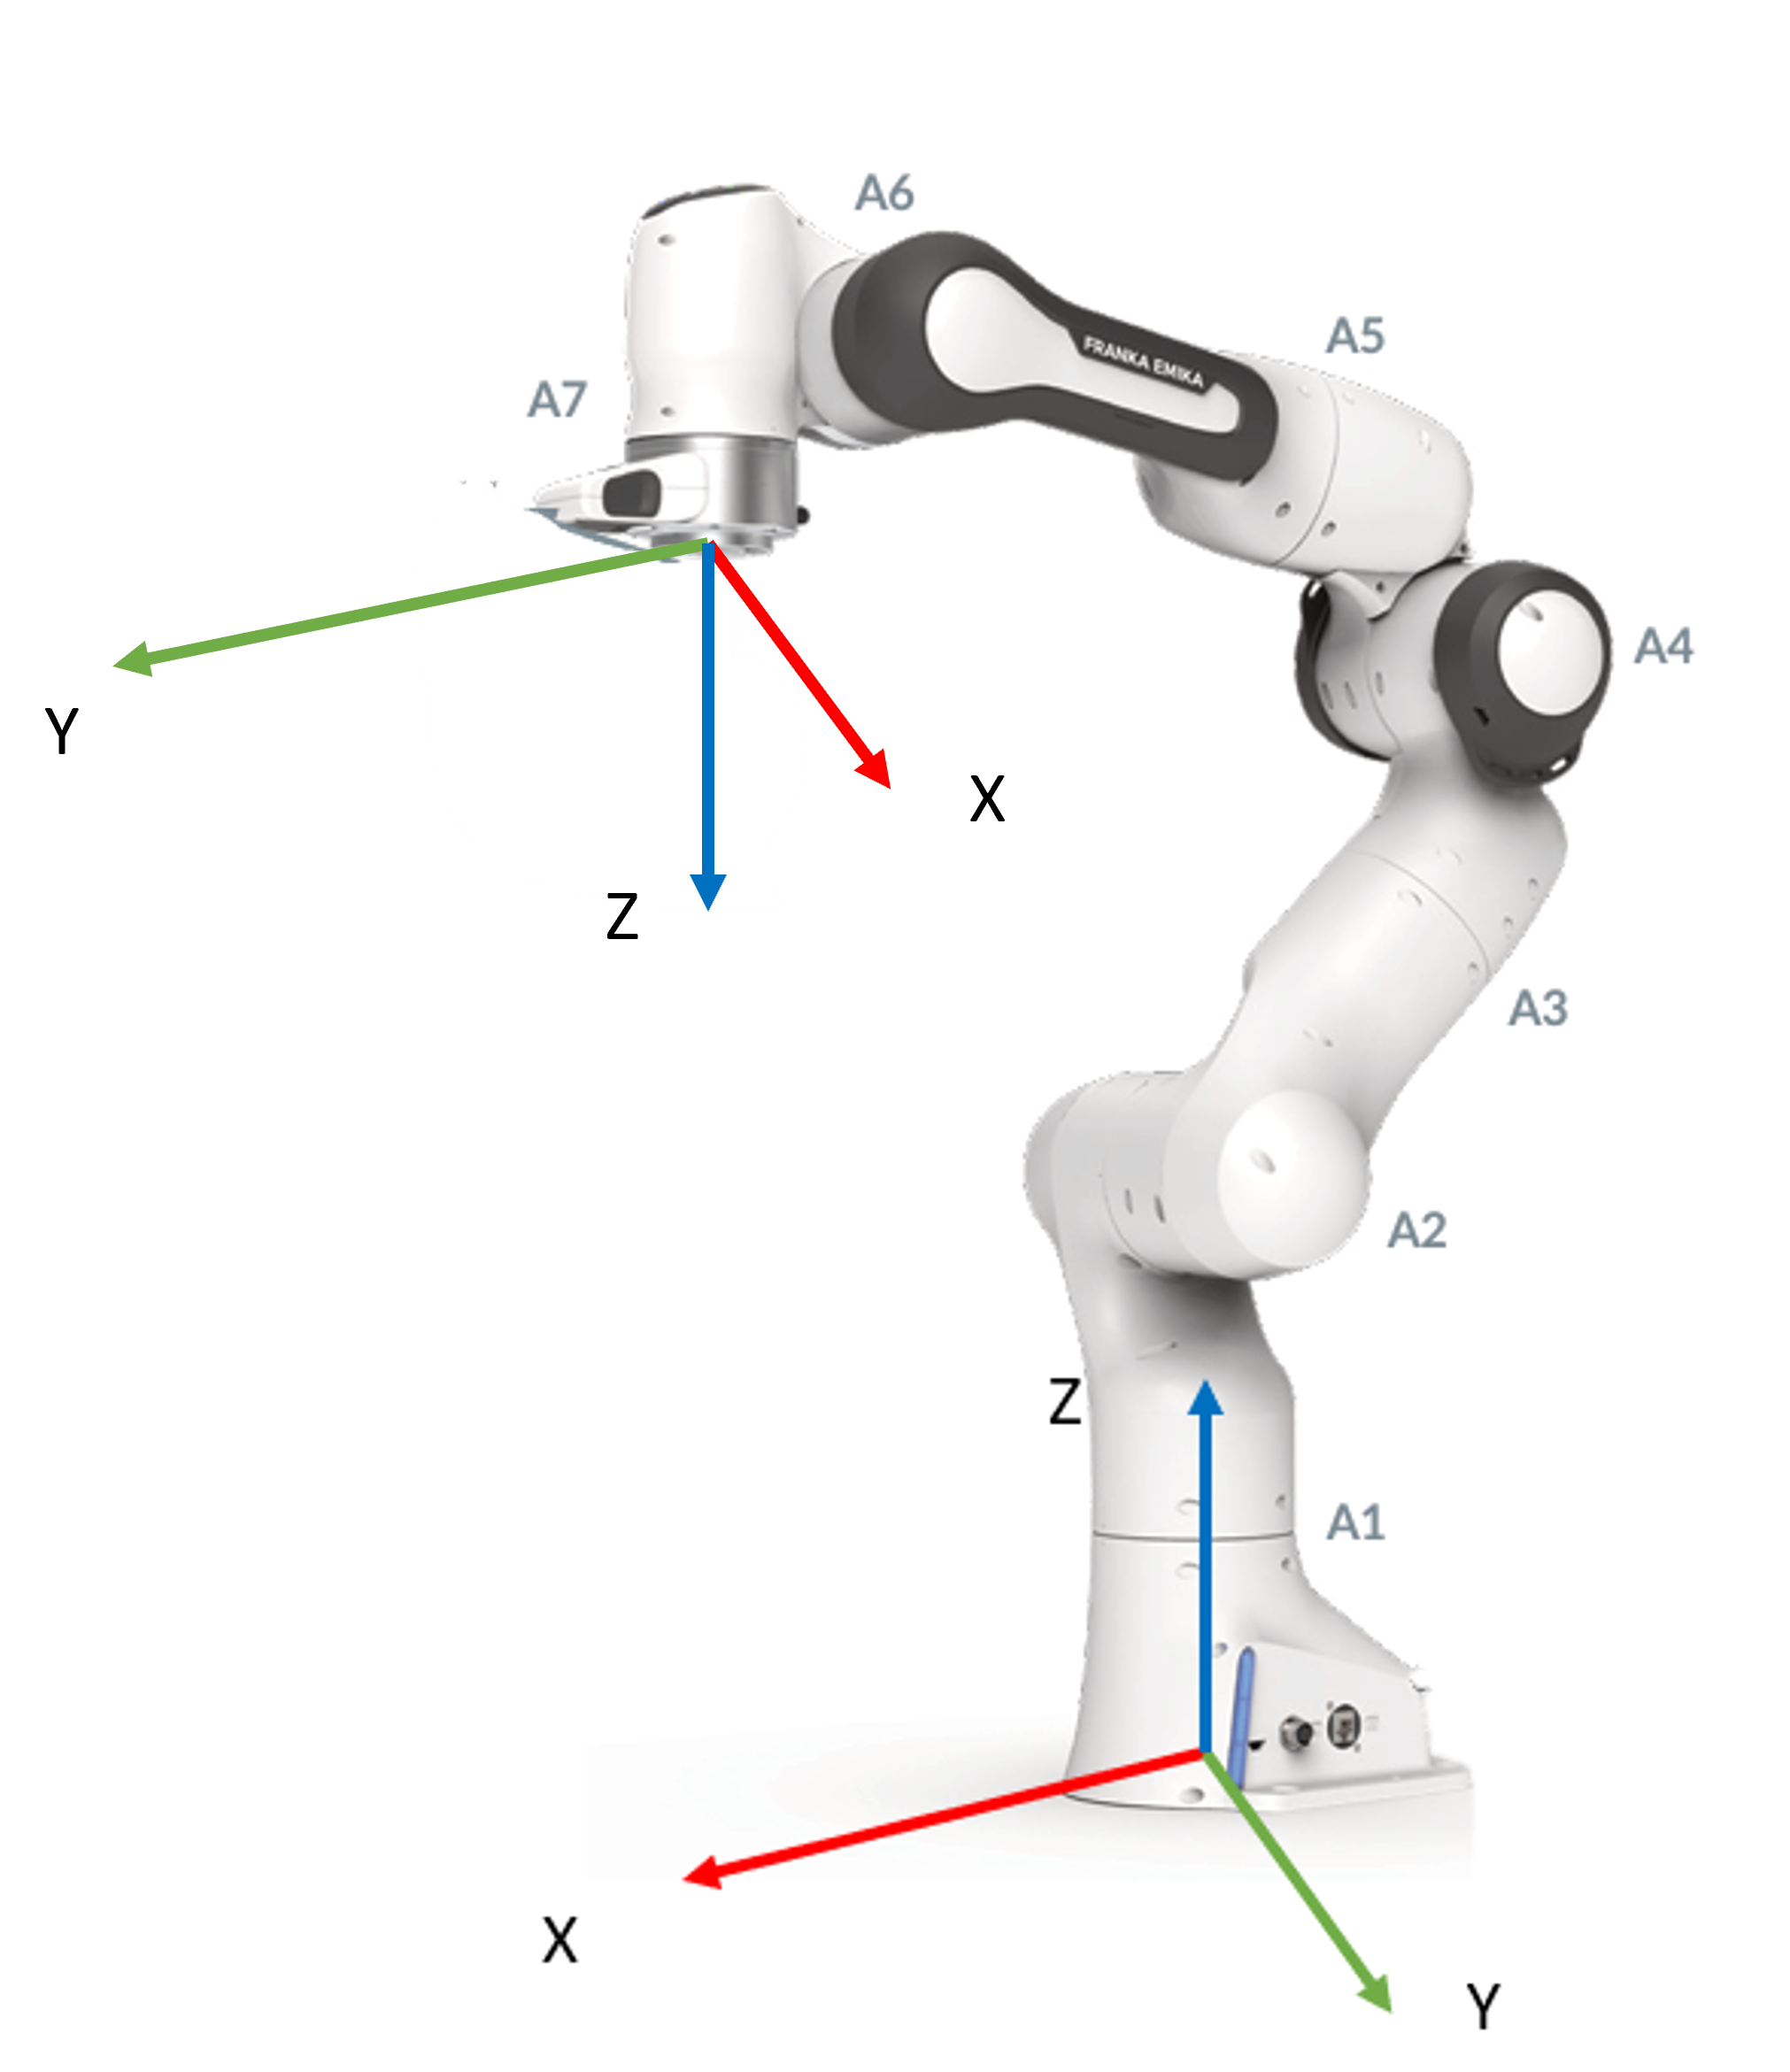
\includegraphics[scale=0.7]{pics/config2.png}
        \caption{The arms and joints of the Panda robot}
    \end{figure}

    Here are the dimensions of the robot.
    \begin{figure}[H]\label{dims}
        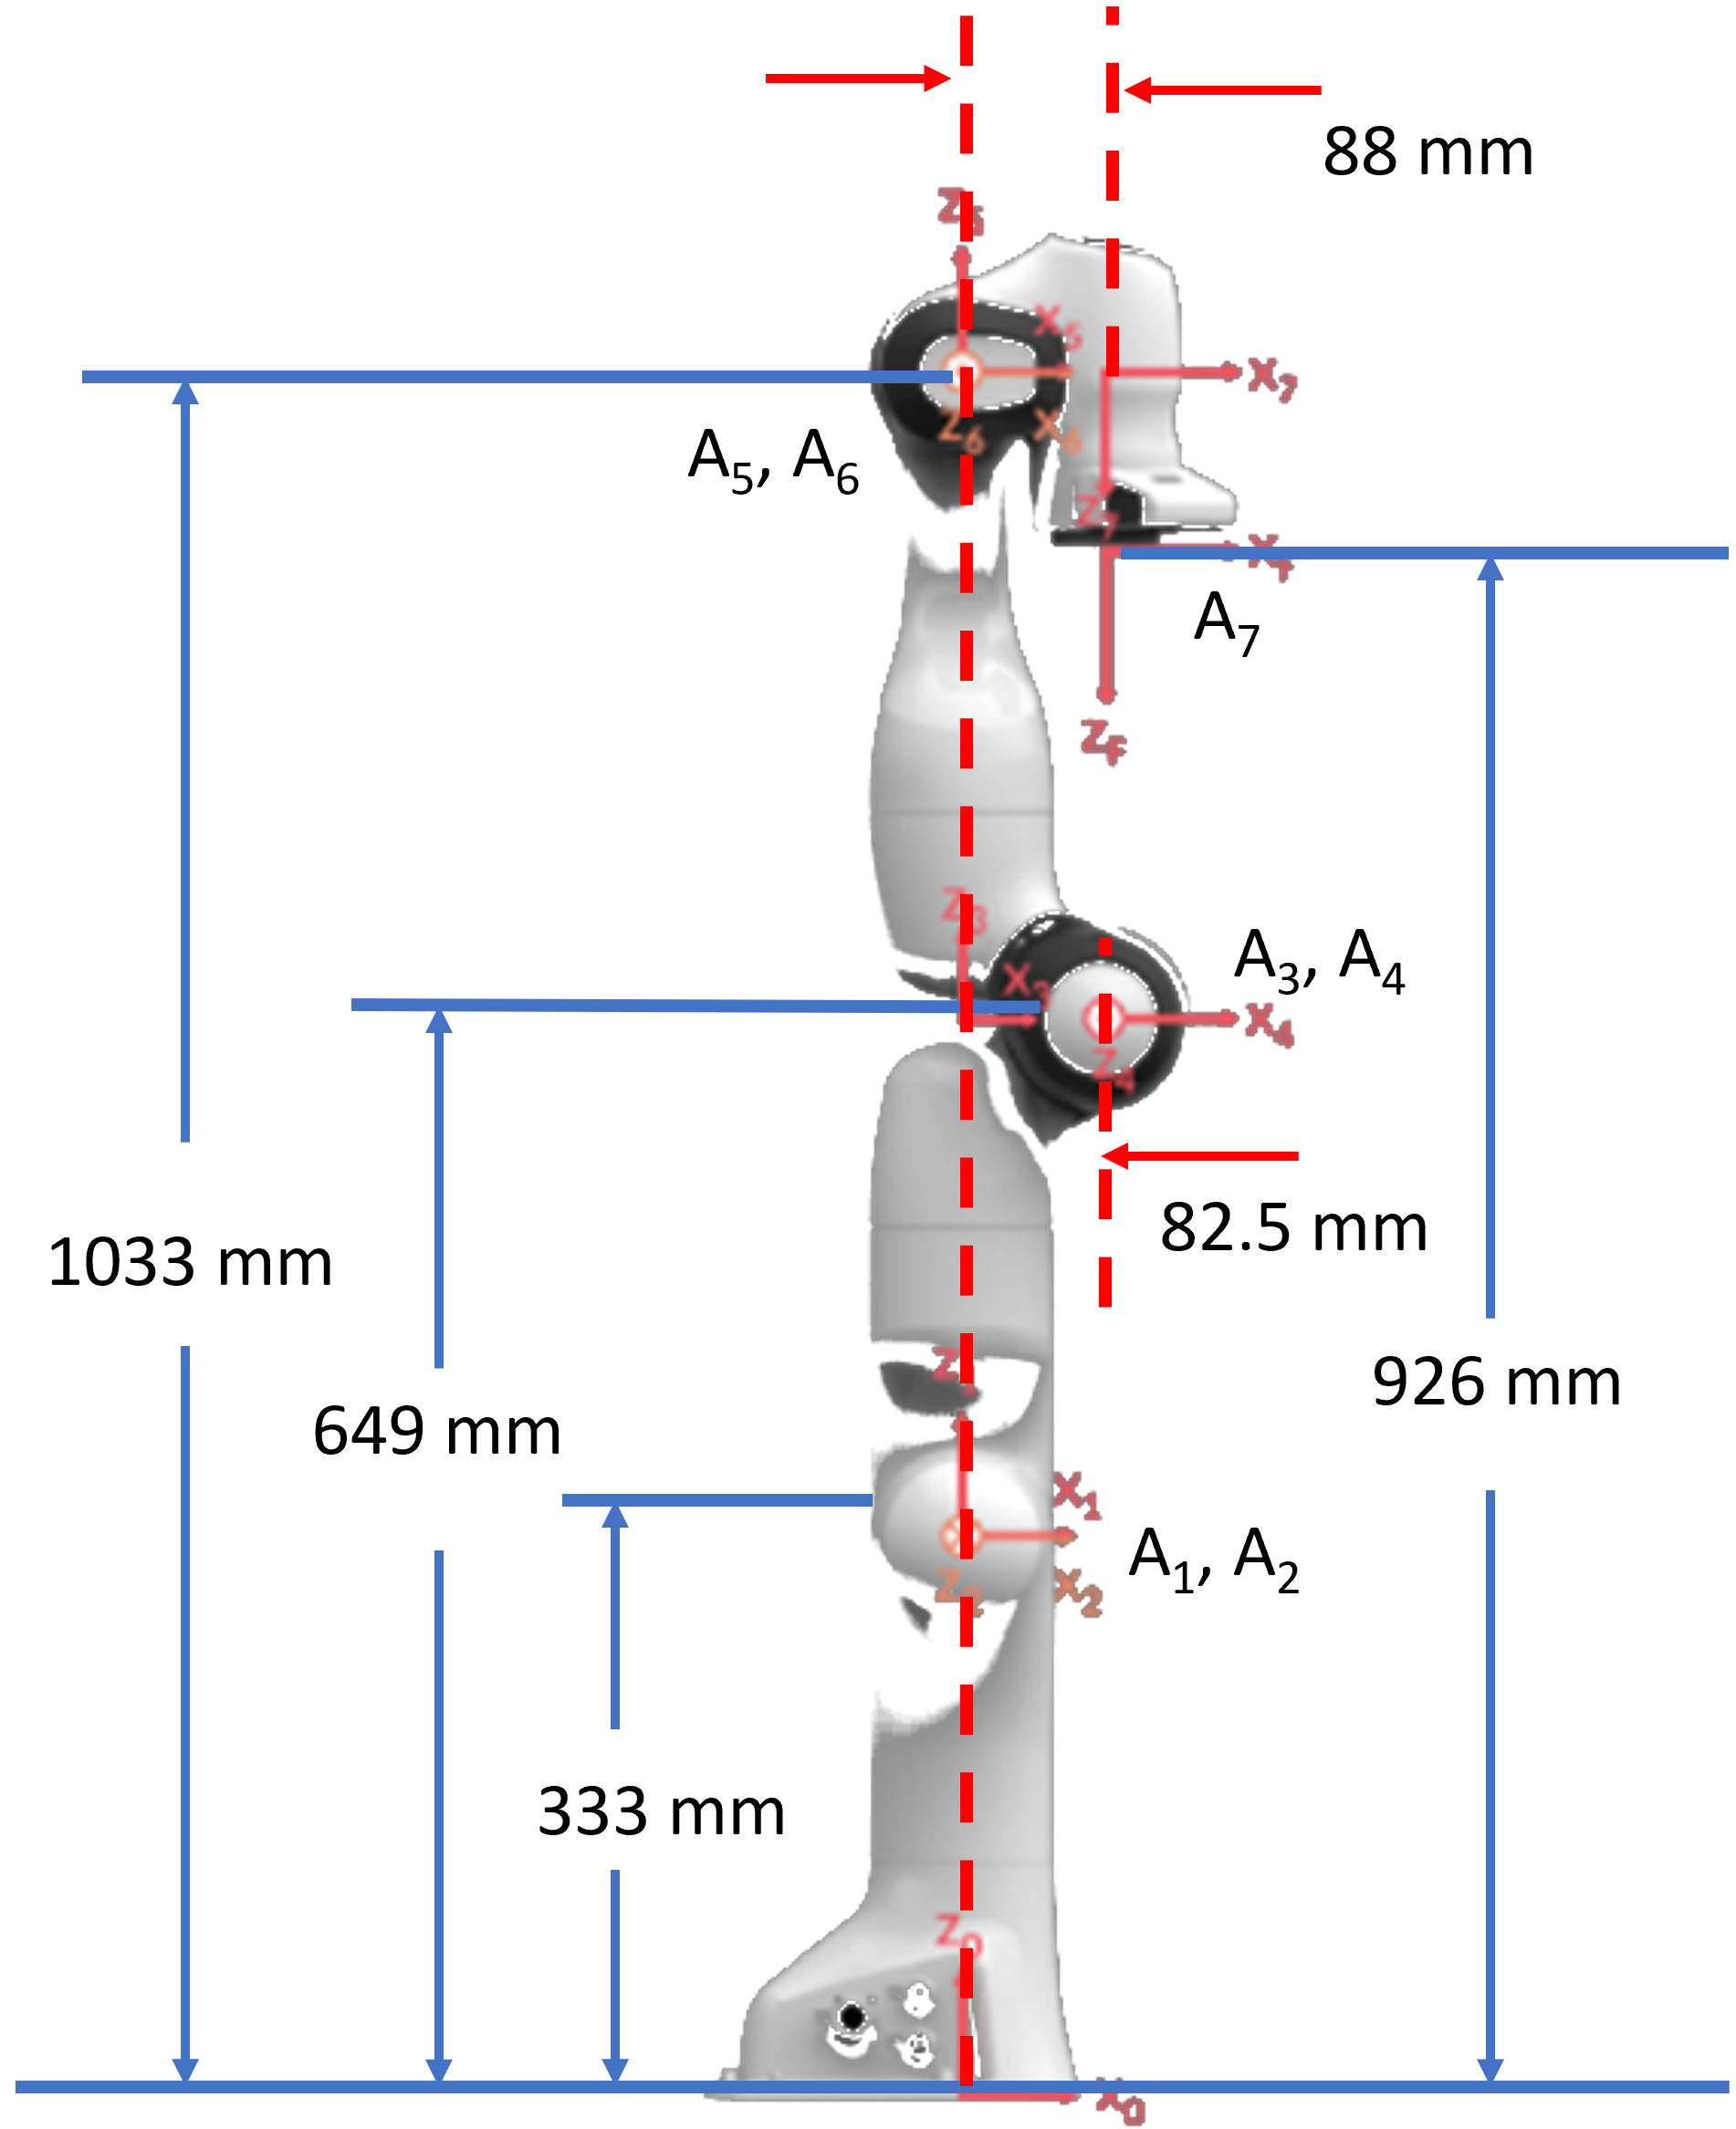
\includegraphics[scale=0.7]{pics/dims.png}
        \caption{The parameters of Panda}
    \end{figure}
	
    The initial configuration is as follows:
    $$M = \begin{bmatrix}
        0 & 1 & 0 & 0.088\\
        1 & 0 & 0 & 0\\
        0 & 0 & -1 & 0.926 \\
        0 & 0 & 0 & 1 \\
    \end{bmatrix}$$
    
    Here is the twist for each joints.
    \begin{center}
        \begin{tabular}{|c|c|c|}
            \hline
            & $\omega_i$ & $v_i$ \\
            \hline
            A1 & $[0, 0, 1]^{T}$ & $[0, 0, 0]^{T}$ \\
            \hline
            A1 & $[0, 1, 0]^{T}$ & $[-0.333, 0, 0]^{T}$ \\
            \hline
            A3 & $[0, 0, 1]^{T}$ & $[0, 0, 0]^{T}$ \\
            \hline
            A4 & $[0, -1, 0]^{T}$ & $[0.649, 0, -0.0825]^{T}$ \\
            \hline
            A5 & $[0, 0, 1]^{T}$ & $[0, 0, 0]^{T}$ \\
            \hline
            A6 & $[0, -1, 0]^{T}$ & $[1.033, 0, 0]^{T}$ \\
            \hline
            A7 & $[0, 0, -1]^{T}$ & $[0, -0.088, 0]^{T}$ \\
            \hline
        \end{tabular}
    \end{center}
    
    Rotation angle restrictions
    \begin{center}
        \begin{tabular}{|c|c|c|}
            \hline
            & min$/^\circ$& max$/^\circ$ \\
            \hline
            A1 & -166 & 166 \\
            \hline
            A1 & -101 & 101 \\
            \hline
            A3 & -166 & 166 \\
            \hline
            A4 & -176 & -4 \\
            \hline
            A5 & -166 & 166 \\
            \hline
            A6 & -1 & 215 \\
            \hline
            A7 & -166 & 166 \\
            \hline
        \end{tabular}
    \end{center}
    
    Joint velocity limits
    \begin{center}
    	\begin{tabular}{|c|c|}
    		\hline
    		& limits $/(^\circ/s)$ \\
    		\hline
    		A1 & 150 \\
    		\hline
    		A1 & 150 \\
    		\hline
    		A3 & 150 \\
    		\hline
    		A4 & 150 \\
    		\hline
    		A5 & 180 \\
    		\hline
    		A6 & 180 \\
    		\hline
    		A7 & 180 \\
    		\hline
    	\end{tabular}
    \end{center}
    
    \section{Programming Assignments}
    \subsection*{a) Find the FK of Panda using the space form of the exponential products}
	The forward kinematics using the Product of Exponentials formula in the space frame is given by:
	\begin{equation}
		T(\theta) = \mathrm{e}^{[S_1]\theta_1} \mathrm{e}^{[S_2]\theta_2} \cdots \mathrm{e}^{[S_n]\theta_n} M
	\end{equation}
	
	This is implemented in \textbf{FK\_space.m}. This function takes the initial configuration of the end-effector, the screw axes and the joint angles as pararmeters and output the coordinates of the end-effector. The declaration of the function is as follows:
    \begin{lstlisting}[style=matlab]
function [T] = FK_space(M, S, theta)
% FK_space calculates the configuration of the end-effector
% Inputs:
%     M is a matrix of 4x4 of initial configuration of end-effector
%     S is a matrix of 6xn of screw axes
%     theta is a joint angle vector nx1
% Outputs:
%   T   - 4x4 the configuration of the end-effector
    \end{lstlisting}
	
    The test program is called \textbf{FK\_space\_test.m}. In this program, we tested several cases of the Panda robot and compare it with the results from matlab robotics toolbox. (Note that the Panda in MATLAB robotics toolbox uses a different initial config of joint 7 with our config. Specifically, when we set the angle of joint 7 to be $-\pi/4$ and all other angles to be zero, we recover our initial configuration.)
	
    This is the screw axes for each joint of Panda
    \begin{center}
        \begin{tabular}{|c|c|}
            \hline
            &  S \\
            \hline
            A1 & $[0, 0, 1, 0, 0, 0]^{T}$ \\
            \hline
            A1 & $[0, 1, 0, -0.333, 0, 0]^{T}$ \\
            \hline
            A3 & $[0, 0, 1, 0, 0, 0]^{T}$ \\
            \hline
            A4 & $[0, -1, 0, 0.649, 0, -0.0825]^{T}$ \\
            \hline
            A5 & $[0, 0, 1, 0, 0, 0]^{T}$  \\
            \hline
            A6 & $[0, -1, 0, 1.033, 0, 0]^{T}$  \\
            \hline
            A7 & $[0, 0, -1, 0, 0.088, 0]^{T}$ \\
            \hline
        \end{tabular}
    \end{center}
    \subsubsection*{Case 1: Forward Reach}
    $$T_d = \begin{bmatrix}
    	0 & 1 & 0 & 0.7\\
    	1 & 0 & 0 & 0\\
    	0 & 0 & -1 & 0.3 \\
    	0 & 0 & 0 & 1 \\
    \end{bmatrix}$$
    
    \subsubsection*{Case 2: Side Reach}
    $$T_d = \begin{bmatrix}
    	0 & 1 & 0 & 0\\
    	1 & 0 & 0 & 0.7\\
    	0 & 0 & -1 & 0.3 \\
    	0 & 0 & 0 & 1 \\
    \end{bmatrix}$$
    
    \subsubsection*{Case 3: Backward Reach}
    $$T_d = \begin{bmatrix}
    	0 & 1 & 0 & -0.6\\
    	1 & 0 & 0 & 0\\
    	0 & 0 & -1 & 0.3 \\
    	0 & 0 & 0 & 1 \\
    \end{bmatrix}$$
    
    \subsubsection*{Case 4: Near singularity}
        $$T_d = \begin{bmatrix}
    	0 & 1 & 0 & 0.088\\
    	1 & 0 & 0 & 0\\
    	0 & 0 & -1 & 0.926 \\
    	0 & 0 & 0 & 1 \\
    \end{bmatrix}$$
    
    
    \subsubsection*{Case 1: Benchmark (Alough it is not feasible due to the angle constraint of joint 4)}
    We set $\theta = \begin{bmatrix}
        0 & 0 & 0 & 0 & 0 & 0 & 0
    \end{bmatrix}^T$. In this case, the configuration should be the initial configuration and it is.
    \subsubsection*{Case 2}
    We set $\theta = \begin{bmatrix}
        0 & -40^o & 0 & -110^o & 0 & 90^o & 0
    \end{bmatrix}^T$. In this case, we try to recover the case in \ref{joints}. Again, we got the same configuration with the MATLAB robotics toolbox.
    $$T = \begin{bmatrix}
        0 & 0.9397 & 0.3420 & 0.312 \\ 1 & 0 & 0 & 0\\ 0 & 0.3420 & -0.9397 & 0.7665\\ 0 & 0 & 0 & 1
    \end{bmatrix}$$
    This is a visualization using MATLAB robotics toolbox.
    \begin{figure}[H]
        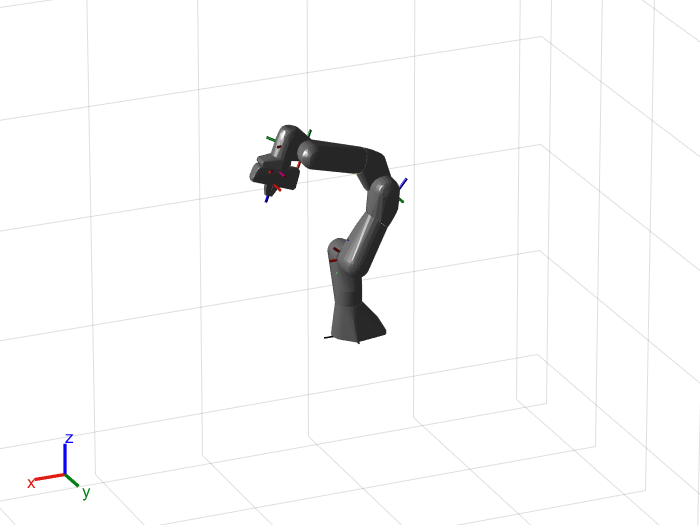
\includegraphics[scale=0.7]{pics/p1t2.png}
    \end{figure}
    
    \subsubsection*{Case 3}
    We set $\theta = \begin{bmatrix}
        20^o & -40^o & 30^o & -110^o & -25^o & 90^o & 10^o
    \end{bmatrix}^T$. This is just a random case to test the rotation along $z$ axis (odd number joints). Again, we got the same configuration with the MATLAB robotics toolbox.
    $$T = \begin{bmatrix}
           -0.3041 &   0.6951  & 0.6515  &  0.1803 \\
        0.7230 &   0.6137 &  -0.3173  &  0.3012\\
        -0.6204  &  0.3745  & -0.6891  &  0.7456\\
        0      &   0     &    0  &  1.0000\\
    \end{bmatrix}$$
    This is a visualization using MATLAB robotics toolbox.
    \begin{figure}[H]
        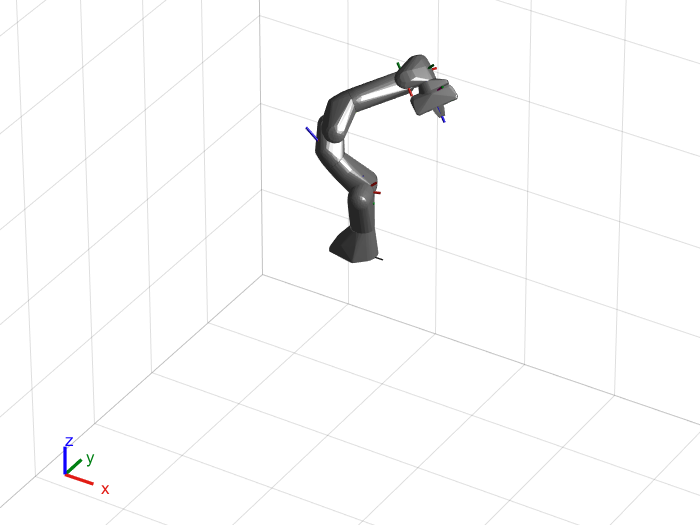
\includegraphics[scale=0.7]{pics/p1t3.png}
    \end{figure}
	
    \subsection*{b) Calculate the space form FK of Panda and represent the defined frames and screw axis graphically}
    This is implemented in \textbf{visualize\_FK\_space.m} (instead of \textbf{FK\_space.m}, because \textbf{FK\_space.m} will be used later for many times to calculate the configuration of the end-effector and we think it is annoyting to plot the graph every time we call the function to get the end-effector).
	
    This function takes the initial configuration of the end-effector, the screw axes, the initial rotation directions, the initial joint positions and the joint angles. The declaration of the function is as follows:
    \begin{lstlisting}[style=matlab]
function visualize_FK_space(M, S, omega, r, theta)
% FK_space calculates the configuration of the end-effector
% Inputs:
%     M is a matrix of 4x4 of initial configuration of end-effector
%     S is a matrix of 6xn of screw axes
%     omega is a matrix of 3xn of initial rotation directions
%     r is a matrix of 3xn of initial joint positions
%     theta is a joint angle vector nx1
% Outputs:
%   T   - 4x4 the configuration of the end-effector
    \end{lstlisting}
    This function does pretty much the same thing with \textbf{FK\_space.m} except it plots the screw axes of each joint at configuration specified by parameter \textbf{theta}.
	
    In the test program \textbf{visualize\_FK\_space\_test.m}. We tested \textbf{Case 2} where \ \ \ $\theta = \begin{bmatrix}
        0 & -40^o & 0 & -110^o & 0 & 90^o & 0
    \end{bmatrix}^T$. Here is the graph generated by it compared with the MATLAB robotics toolbox.
    \begin{figure}[H]
        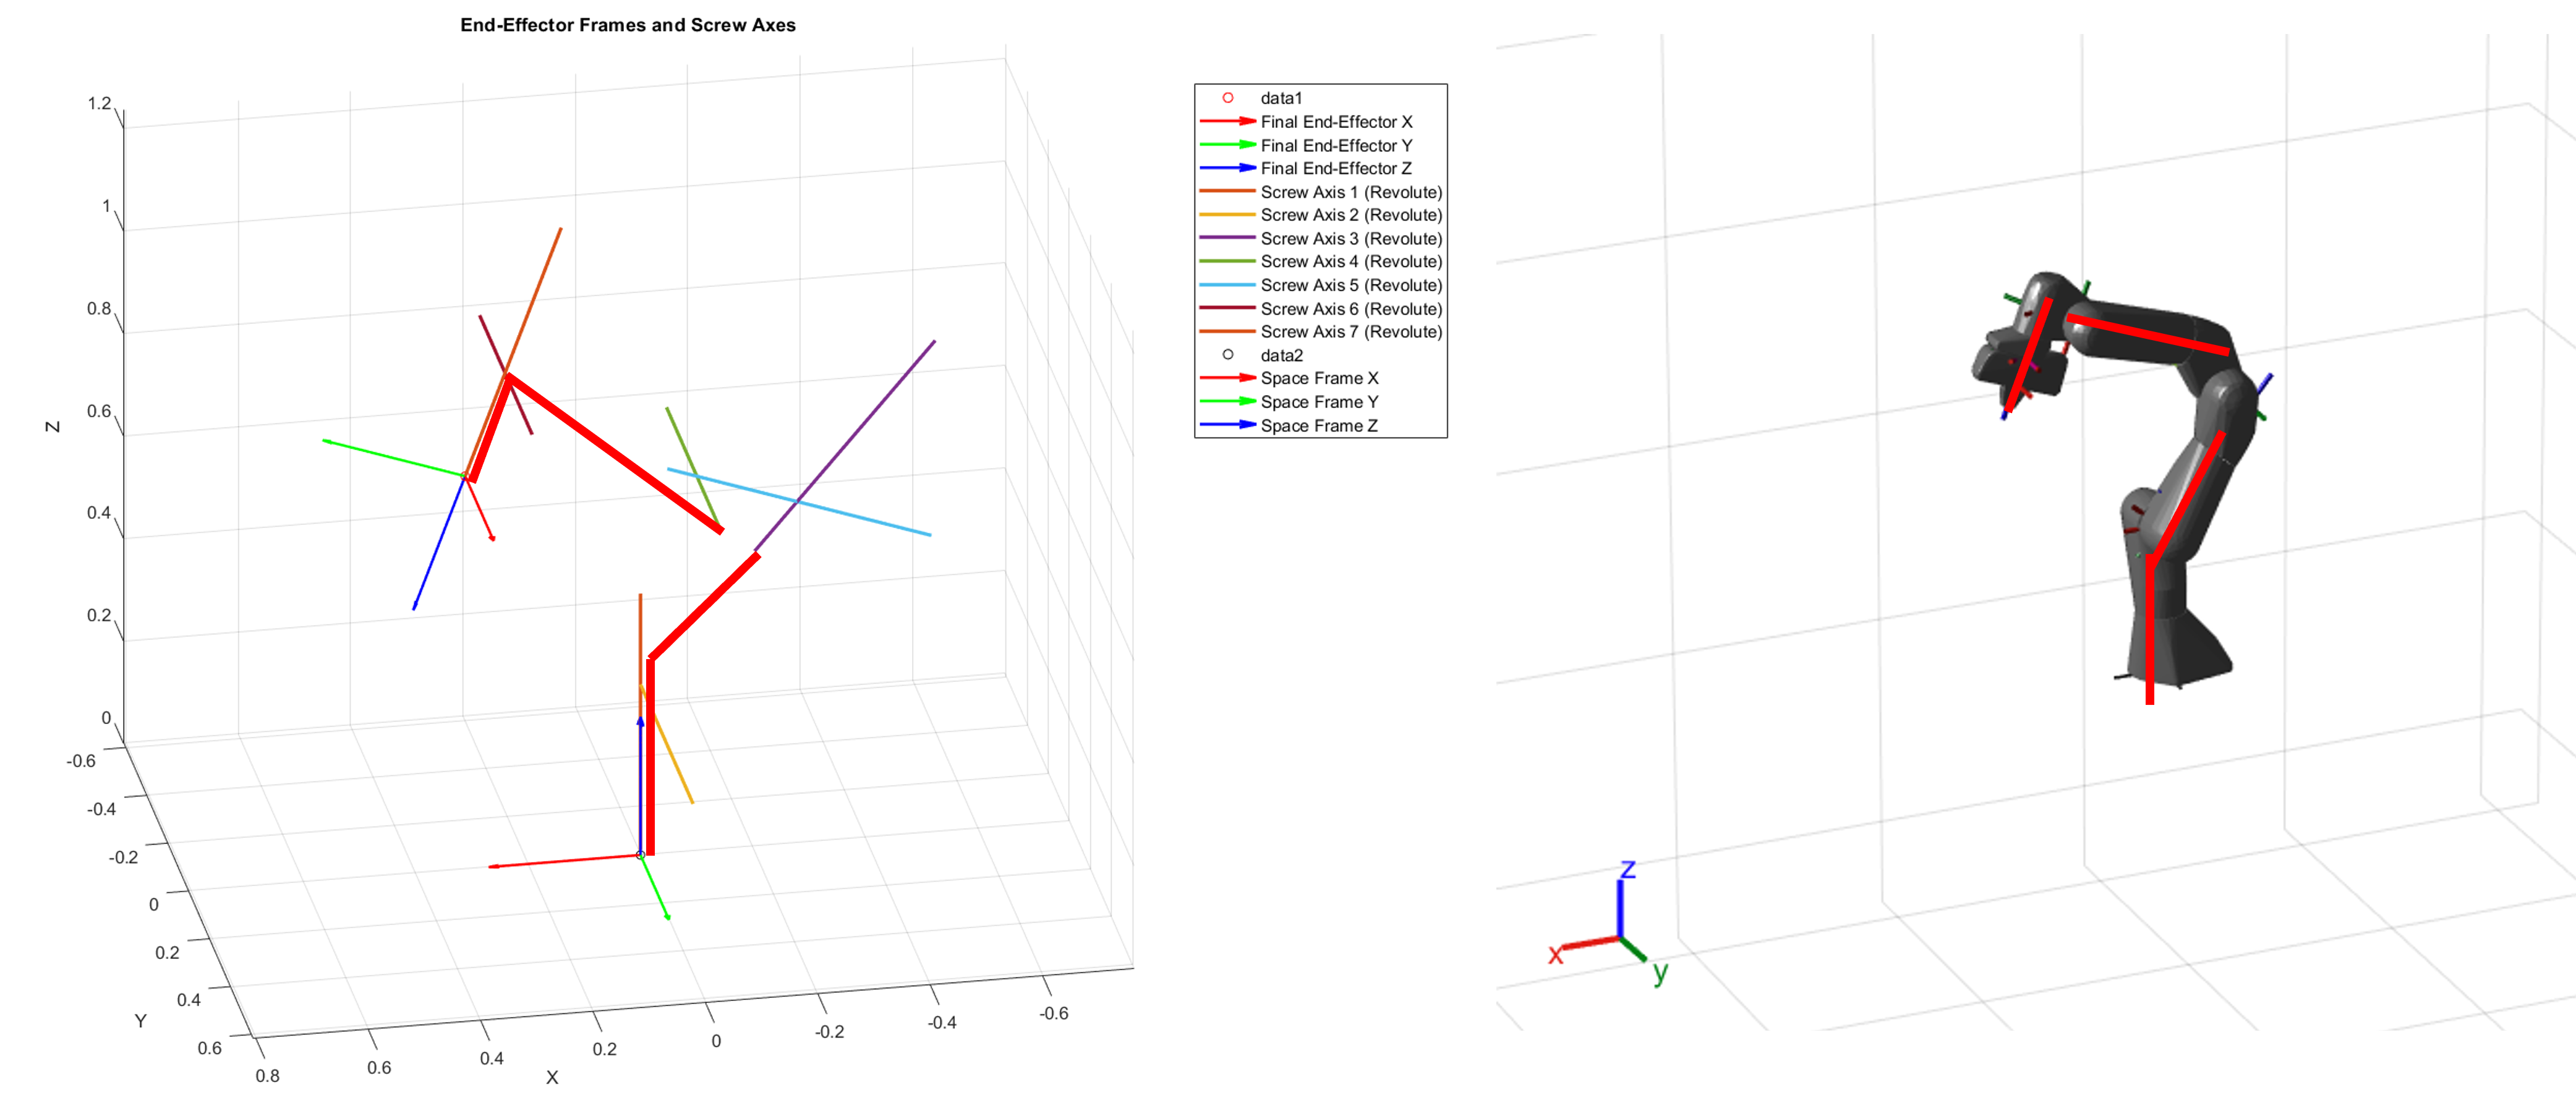
\includegraphics[scale=0.5]{pics/p2t1.png}
    \end{figure}
    \subsection*{c) Repeat (a) and (b) for body form FK}
    This is implemented in \textbf{FK\_body.m}. This function takes the initial configuration of the end-effector, the screw axes in body form and the joint angles as parameters and outputs the coordinates of the end-effector.
    
    This is the screw axes in body form for each joint of Panda
    \begin{center}
        \begin{tabular}{|c|c|}
            \hline
            &  B \\
            \hline
            A1 & $[0, 0, -1, 0.088, 0, 0]^{T}$ \\
            \hline
            A1 & $[1, 0, 0, 0, 0.593, 0.088]^{T}$ \\
            \hline
            A3 & $[0, 0, -1, 0.088, 0, 0]^{T}$ \\
            \hline
            A4 & $[-1, 0, 0, 0, -0.277, -0.0055]^{T}$ \\
            \hline
            A5 & $[0, 0, -1, 0.088, 0, 0]^{T}$  \\
            \hline
            A6 & $[-1, 0, 0, 0, 0.1070, -0.088]^{T}$  \\
            \hline
            A7 & $[0, 0, 1, 0, 0, 0]^{T}$ \\
            \hline
        \end{tabular}
    \end{center}
	
    The test program is called \textbf{FK\_body\_test.m} where the three cases in \textbf{FK\_space\_test.m} were used and validated against the results here.
    
    Similarly, we have the \textbf{visualize\_FK\_body.m} to plot the defined frames and screw axes graphically and the corresponding test program \textbf{visualize\_FK\_body\_test.m} and we get the same results.
    
    \subsection*{d) Find the space and body form Jacobian of Panda}
    We use formulae

    $$\mathcal{V}_s = \begin{bmatrix}
    J_{s1} & J_{s2} & \cdots & J_{sn} 
\end{bmatrix}  \begin{bmatrix}
\dot{\theta}_1 \\ \dot{\theta}_2 \\ \vdots \\ \dot{\theta}_n
\end{bmatrix}$$
    where 
\begin{align*}
    J_{s1} &= \mathcal{S}_1 \\
    J_{s2} &= \text{Ad}_{e^{[S_1]\theta_1}} \mathcal{S}_2 \\
    \cdots
\end{align*}

    Similarly, for body form Jacobian:
$$\mathcal{V}_b = \begin{bmatrix}
    J_{b1} & J_{b2} & \cdots & J_{bn} 
\end{bmatrix}  \begin{bmatrix}
    \dot{\theta}_1 \\ \dot{\theta}_2 \\ \vdots \\ \dot{\theta}_n
\end{bmatrix}$$
    where 
\begin{align*}
    J_{bn} &= \mathcal{B}_n \\
    J_{b,{n-1}} &= \text{Ad}_{e^{-[B_n]\theta_n}} \mathcal{B}_{n-1} \\
    \cdots
\end{align*}
	
    \subsection*{e) Write functions to calculate the space and body form Jacobians of the robot}
These are implemented in \textbf{J\_space.m} and \textbf{J\_body.m} for space and body form Jacobians, respectively. For the space-form Jacobian, the function takes the screw axes in body form and the joint angles as parameters and outputs the space-form Jacobian of the end-effector. The declaration of the function is as follows:
    \begin{lstlisting}[style=matlab]
function [J] = J_space(S, theta)
% J_SPACE Calculate the space Jacobian matrix for a serial robot
%
% Inputs:
%   S     - 6xn matrix of normalized twists, where each column is a 6x1 twist
%          vector [omega; v] representing the joint axis in space frame
%   theta - nx1 vector of joint angles/positions
%
% Output:
%   J     - 6xn space Jacobian matrix
\end{lstlisting}
    The body form of the Jacobian is similar.
    \subsubsection*{Case 1-3}
    The test program is called \textbf{J\_space\_body\_test.m} to test the two functions. Again, we used the three cases mentioned earlier. The test is two-fold. Firstly, we use cross-validation of the space-form Jacobian and body-form Jacobian with the following formulae:
    \[J_s = \text{Ad}_{T_{sb}} J_b\]
    Secondly, we validate our results with the results from MATLAB robotics toolbox. Note that the Jacobian calculated by \textbf{geometricJacobian} is actually analytic form Jacobian, as stated in \cite{Lynch_Park_2017}. And it can be transformed to body-form Jacobian using the following formulae:
    \[J_a = \begin{bmatrix}
        R_{sb} & 0 \\
        0 & R_{sb}
    \end{bmatrix} J_b\]
    \subsubsection*{Case 4}
    We further tested our program using the definition of Jacobian matrix.
    \begin{equation}
        J(\theta)\Delta \theta = \text{Ad}(\Delta T)
    \end{equation}
    or
    \begin{equation}
        J(\theta)\Delta \theta = \text{Ad}_{T(\theta + \Delta \theta) / T(\theta)}
    \end{equation}
    For example, when $\theta = \begin{bmatrix}
        0 & -40^o & 0 & -110^o & 0 & 90^o & 0
    \end{bmatrix}^T$ and $\Delta\theta$ is chosen to be \ \ \ $\theta = \pi/200\begin{bmatrix}
        1 & 1 & 1 & 1 & 1 & 1 & 1
    \end{bmatrix}^T$. We get
    \begin{equation}
        \text{Ad}_{T(\theta + \Delta \theta) / T(\theta)} = \begin{bmatrix}
                0.0106 &   -0.0154 &   0.0185 &   0.0175 &   0.0172 &  -0.0009
        \end{bmatrix}^T
    \end{equation}
    And 
    \begin{equation}
        J(\theta)\Delta \theta = \begin{bmatrix}
                0.0100 &   -0.0157 &   0.0184 &   0.0178 &   0.0167 &  -0.0008
        \end{bmatrix}^T
    \end{equation}
    which are very close, as expected.
    \subsection*{f) Write a function \textbf{singularity.m} to calculate the singularity configurations of the robot}
    According to \cite{Hepanda} and \cite{Tittelpanda}, Panda's singularity exists when joints 1, 3 and 5 aligned and the robot would lose two DoF, leaving it with just 5-DoF and incapable of certain motion. It is acchieved when $\theta = \begin{bmatrix}
        0 & 0 & 0 & 0 & 0 & 0 & 0
    \end{bmatrix}^T$, as shown in the following picture. 
    \begin{figure}[H]
        \centering
        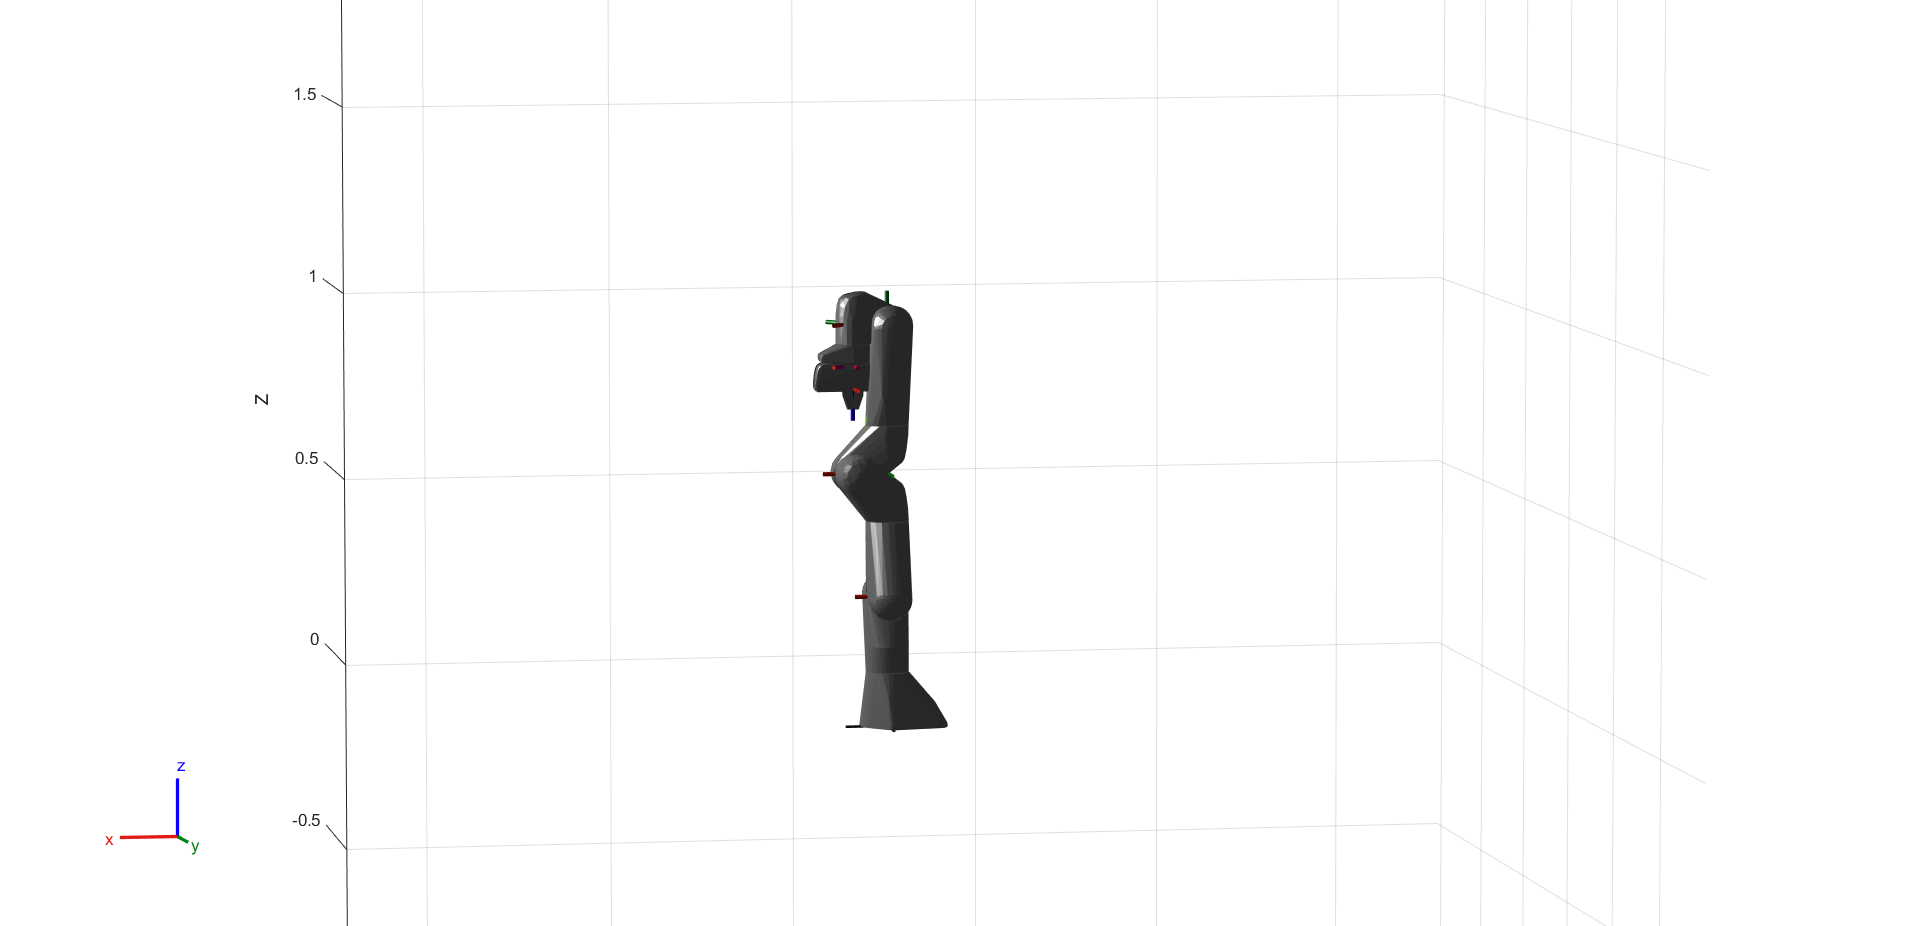
\includegraphics[width=\linewidth]{pics/singularity.png}
        \caption{Singularity case}
        \label{fig:enter-label}
    \end{figure}
    This could be validated using the rank of Jacobian matrix. Furthermore, we can use function \textbf{jsingu} to show which columns are linearly dependent.
    \begin{lstlisting}[style=matlab]
         5

2 linearly dependent joints:
  q3 depends on: q1 
  q5 depends on: q1 
    \end{lstlisting}

    \subsection*{g) Write functions that }
    \subsubsection*{a) show/plot the manipulability ellipsoids for the angular and linear velocities and their axes}
    The two functions are implemented in \textbf{ellipsoid\_plot\_angular.m} and \textbf{ellipsoid\_plot\_linear.m}, respectively. And their test program with sufix \textbf{\_test}.
    
    When $\theta = \begin{bmatrix}
        0 & 0 & 0 & 0 & 0 & 0 & 0
    \end{bmatrix}^T$, we know it is at singularity and the ellipsoid should be a plane for angular velocities. (Because we lost the freedom in angular motions instead of linear motions) And so did our program got.
    \begin{figure}[H]
        \centering
        \begin{minipage}{0.45\textwidth}
            \centering
            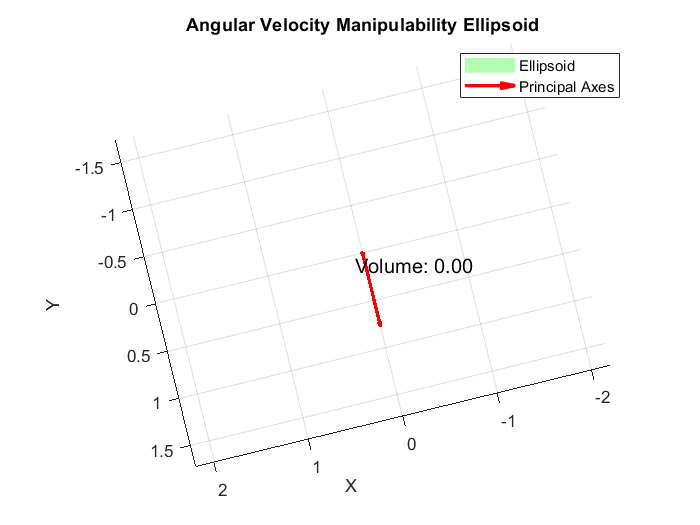
\includegraphics[width=\textwidth]{pics/pga1a.png} % Replace with your image file
            \caption{Angular Velocity Manipulability Ellipsoid}
            \label{fig:pga1a}
        \end{minipage}
        \hfill
        \begin{minipage}{0.45\textwidth}
        \centering
            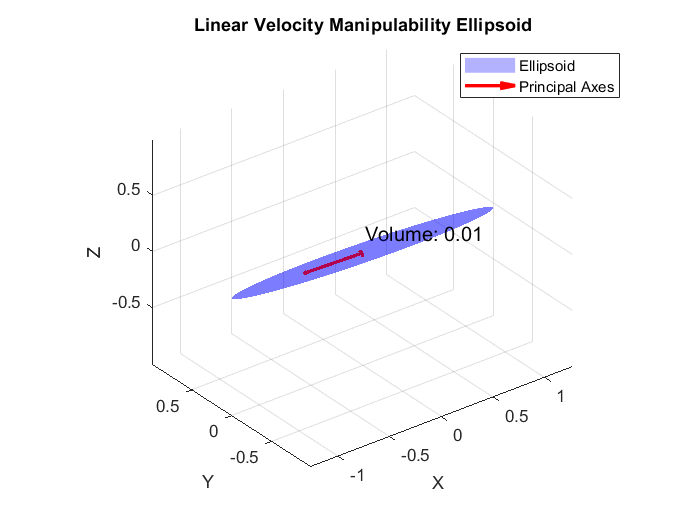
\includegraphics[width=\textwidth]{pics/pga1l.png} % Replace with your image file
            \caption{Linear Velocity Manipulability Ellipsoid}
            \label{fig:pga1l}
        \end{minipage}
    \end{figure}

    The following are the results when $\theta = \begin{bmatrix}
        0 & -40^o & 0 & -110^o & 0 & 90^o & 0
    \end{bmatrix}^T$ which is not at singularity.
    \begin{figure}[H]
        \centering
        \begin{minipage}{0.45\textwidth}
            \centering
            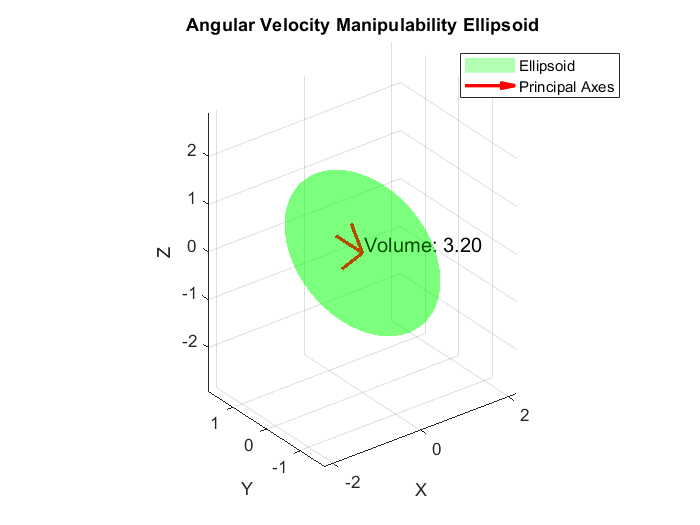
\includegraphics[width=\textwidth]{pics/pga2a.png} % Replace with your image file
            \caption{Angular Velocity Manipulability Ellipsoid}
            \label{fig:pga2a}
        \end{minipage}
        \hfill
        \begin{minipage}{0.45\textwidth}
        \centering
            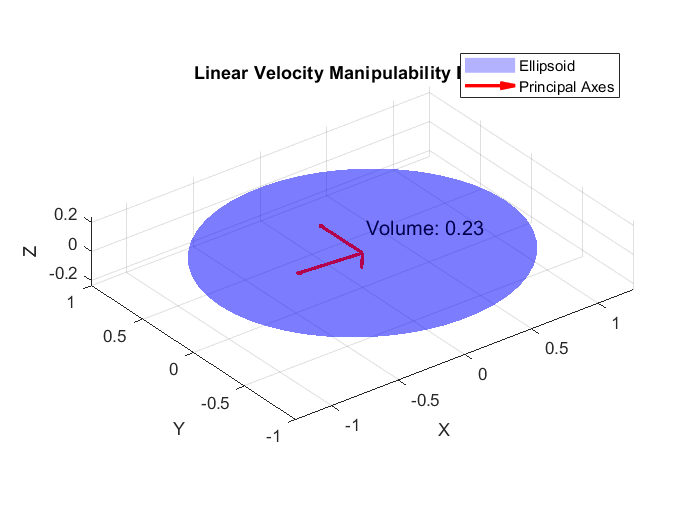
\includegraphics[width=\textwidth]{pics/pga2l.png} % Replace with your image file
            \caption{Linear Velocity Manipulability Ellipsoid}
            \label{fig:pga2l}
        \end{minipage}
    \end{figure}
    \subsubsection*{b) Calculate the isotropy, condition number and volume of the ellipsoids}
    \begin{table}[H]
    \centering
    \begin{tabular}{|p{1.5cm}|c|c|c|c|}
        \hline
        \multirow{2}{*}{ } & \multicolumn{2}{|c|}{Case 1\newline \(\theta = \begin{bmatrix}
        0 & 0 & 0 & 0 & 0 & 0 & 0 \end{bmatrix}^T\)} & \multicolumn{2}{|c|}{Case 2 $\theta = \begin{bmatrix}
        0 & -40^o & 0 & -110^o & 0 & 90^o & 0
    \end{bmatrix}^T$} \\ \cline{2-5}
         &  space-form Jacobian & body-form Jacobian & space-form Jacobian & body-form Jacobian\\ \hline
        isotropy & Inf & Inf & 10.90 & 9.75 \\ \hline
        condition number & Inf & Inf & 118 & 95 \\ \hline
        volume of the ellipsoid & 0 & 0 & 0.0929 & 0.0929 \\ \hline
    \end{tabular}
    \caption{test results for isotropy, condition number and volume of the ellipsoids}
    \label{tab:pgb}
    \end{table}
    From the test results, we observe that 
    \begin{enumerate}
        \item when \(\theta = \begin{bmatrix}
        0 & 0 & 0 & 0 & 0 & 0 & 0 \end{bmatrix}^T\), the robot is at singularity. Therefore, the isotropy and condition number is infinity which is as expected.
        \item when \(\theta = \begin{bmatrix} 0 & -40^o & 0 & -110^o & 0 & 90^o & 0 \end{bmatrix}^T\), the isotropy and condition number are greater than 1. The volume by calculated by space-form Jacobian and body-form Jacobian are the same.
    \end{enumerate}

    \subsection*{h) Use the derived forward kinematics and Jacobians, write a function that uses the iterative numerical inverse kinematics algorithm to control the robot from arbitrary configuration a to configuration b}
    Here, we used the space-form Jacobian to conduct inverse kinematics. The update formulae is
    \begin{algorithm}[H]
    	\caption{Iteration Framework for All Inverse Kinematics Methods}
    	\label{alg:dls_ik}
    	\begin{algorithmic}[1]
    		\State \textbf{Input:} 
    		\State \quad $M$: 4$\times$4 home configuration matrix
    		\State \quad $S$: 6$\times n$ matrix of normalized twists in space frame
    		\State \quad $T_d$: 4$\times$4 desired end-effector configuration matrix
    		\State \quad $\mathbf{\theta}_0$: $n\times 1$ initial joint angles
    		\State \quad $\epsilon$: Error tolerance (default: $10^{-4}$)
    		\State \textbf{Output:} 
    		\State \quad $\mathbf{\theta}^*$: $n\times 1$ joint angles achieving $T_d$ (or approximation)
    		\State 
    		\State \textbf{Initialization:}
    		\State $\mathbf{\theta} \gets \mathbf{\theta}_0$ \Comment{Set initial joint angles}
    		\State $\mathbf{e} \gets \mathbf{1}_{n \times 1}$ \Comment{Initialize error vector}
    		\While{$\|\mathbf{e}\| > \epsilon$} \Comment{Check convergence}
    		\State $T_c \gets FK_{space}(M, S, \mathbf{\theta})$ \Comment{Compute current pose via forward kinematics}
    		\State $\mathbf{e} \gets Ad(T_c) \cdot \log(T_c^{-1} T_d)$ \Comment{Compute twist error in space frame}
    		\State $J \gets J_{space}(S, \mathbf{\theta})$ \Comment{Compute space Jacobian}
    		\State $\Delta \mathbf{\theta} \gets f(\mathbf{e})$ \Comment{Different update formulaes}
    		\State $\mathbf{\theta} \gets \mathbf{\theta} + \Delta \mathbf{\theta}$ \Comment{Update joint angles}
    		\EndWhile
    		\State \textbf{return} $\mathbf{\theta}$ \Comment{Final joint configuration}
    	\end{algorithmic}
    \end{algorithm}
    \begin{align}
        e &= \text{Ad}_{T_{sb}} [T_{sb}^{-1}  T_{sd}]\\ \nonumber
        \Delta\theta &= J^\dagger e \\ \nonumber
        \theta &\leftarrow \theta + \Delta\theta \nonumber
    \end{align}
    The declaration of the function is as follows:
    \begin{lstlisting}[style=matlab]
function theta = J_inverse_kinematics(M, S, T_desired, theta_init, epsilon)
% J_inverse_kinematics Solve inverse kinematics using iterative Newton-Raphson method
%
% Inputs:
%   B          - 6xn matrix of normalized twists in body frame
%   M          - 4x4 home configuration matrix
%   T_desired  - 4x4 desired end-effector configuration matrix
%   theta_init - nx1 initial guess for joint angles
%   epsilon    - Error tolerance (default: 1e-4)
%
% Outputs:
%   theta   - nx1 vector of joint angles that achieve T_desired
%   success - Boolean indicating whether algorithm converged
%
% Note:
%   Uses Newton-Raphson iteration with space Jacobian.
    \end{lstlisting}
    The test program is called \textbf{J\_inverse\_kinematics\_test.m} to test the function.
    \subsection*{Case 1}
    In this case, we set $T_{sd}$ (which is random)
    \begin{equation}
        T_{sd} = \begin{bmatrix}
            0.3862 & -0.2690 & -0.8823 & 0.4225\\
            0.8917 & 0.3535 & 0.2826 & 0.3776\\
            0.2359 & -0.8959 & 0.3764 &  -0.0874\\
            0 & 0 & 0 & 1.00
        \end{bmatrix}
    \end{equation}
    And we use random initial \(\theta = \begin{bmatrix}
        0 & -\pi/2 & 0 & -\pi/2 & 0 & 0 & 0 \end{bmatrix}^T\). (Note to keep to within the joint angle constraints). The followings pictures shows the initial and desired configuration of the robot.
    \begin{figure}[H]
        \centering
        \begin{minipage}{0.45\textwidth}
            \centering
            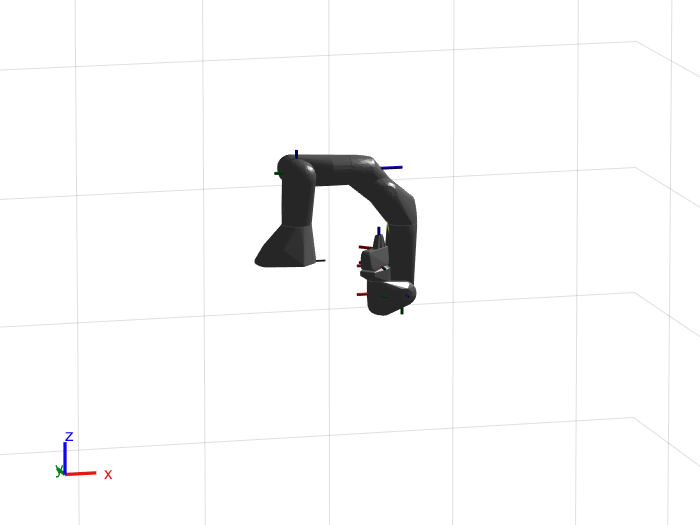
\includegraphics[width=\textwidth]{pics/ph1a.png} % Replace with your image file
            \caption{Initial Configuration}
            \label{fig:ph1a}
        \end{minipage}
        \hfill
        \begin{minipage}{0.45\textwidth}
        \centering
            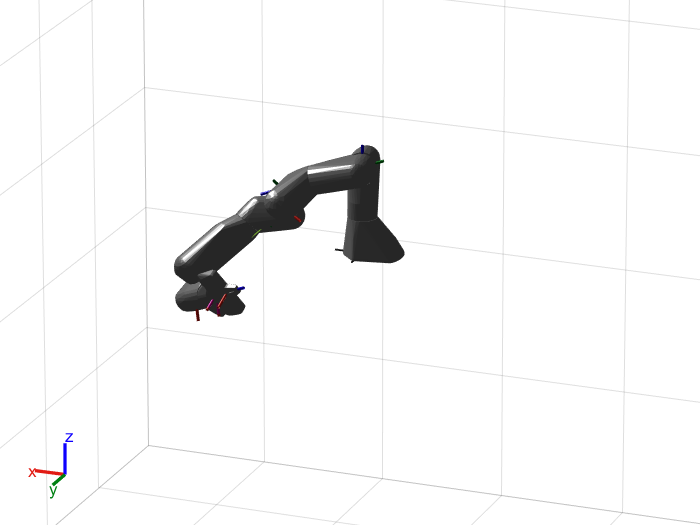
\includegraphics[width=\textwidth]{pics/ph1b.png} % Replace with your image file
            \caption{Desired Configuration}
            \label{fig:ph1b}
        \end{minipage}
    \end{figure}
    This program output \(\theta = \begin{bmatrix} 0.5642 & 1.8297 & -0.1648 & -0.6123 & 1.3935 & 0.7434 & 0.4404 \end{bmatrix}^T\) and exactly the same final configuration of the end-effector.
    
    \subsection*{Case 2}
    In this case, we test the robustness of the program by setting the desired configuration to be very close to singularity. (\(\theta = \begin{bmatrix}
        0.01 & 0.02 & 0.03 & -0.1 & 0.05 & 0.06 & 0.07 \end{bmatrix}^T\)) The desired configuration is
    \begin{equation}
        T_{sd} = \begin{bmatrix}
            -0.0198 & 0.9980 & -0.0601 & 0.1339\\
            0.9998 & 0.0199 & 0.0012 & 0.0097\\
            0.0024 & -0.0601 & -0.9982 & 0.9263\\
            0 & 0 & 0 & 1.00
        \end{bmatrix}
    \end{equation}
    And the condition number at this place is \(1621.7\).
    
    And we use initial guess \(\theta = \begin{bmatrix}
        0 & 1 & 0 & -0.5 & 0 & 0 & 0 \end{bmatrix}^T\). The followings pictures shows the initial and desired configuration of the robot.
    \begin{figure}[H]
        \centering
        \begin{minipage}{0.45\textwidth}
            \centering
            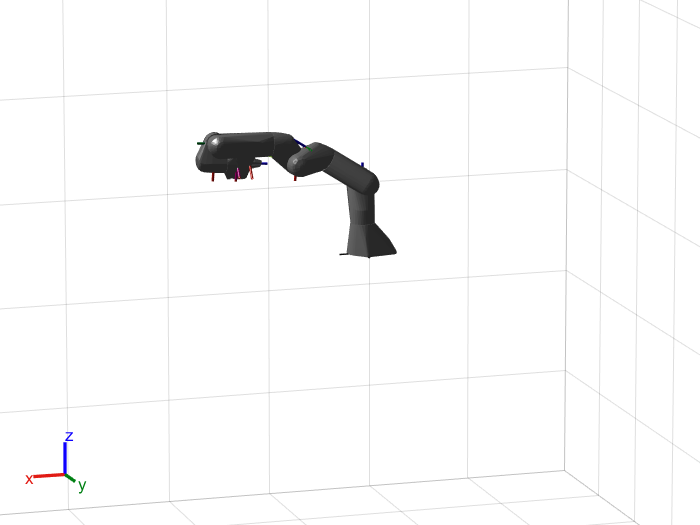
\includegraphics[width=\textwidth]{pics/ph2a.png} % Replace with your image file
            \caption{Initial Configuration}
            \label{fig:ph2a}
        \end{minipage}
        \hfill
        \begin{minipage}{0.45\textwidth}
        \centering
            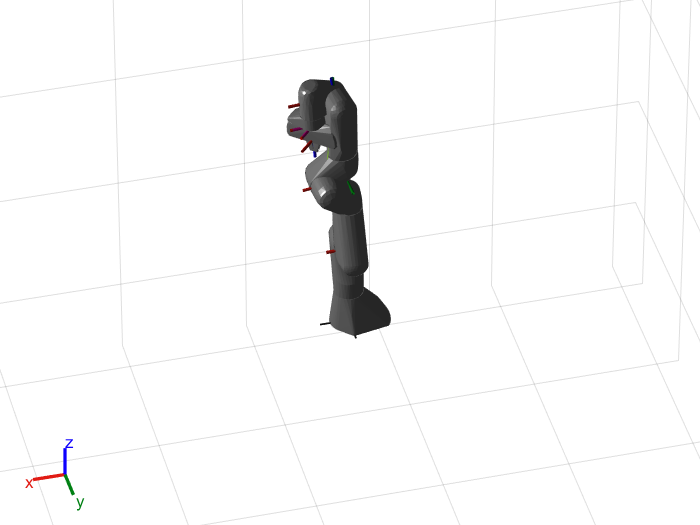
\includegraphics[width=\textwidth]{pics/ph2b.png} % Replace with your image file
            \caption{Desired Configuration}
            \label{fig:ph2b}
        \end{minipage}
    \end{figure}
    This program output exactly the same final configuration of the end-effector and \ \ \ \(\theta = \begin{bmatrix} -3.2855 & 12.1961 & 5.6213 & 18.3704 & 2.4528 & -6.5735 & 4.8143 \end{bmatrix}^T\). The \(\theta\) exceeds the joint angles limits and needed further modification.

    \subsection*{i) Use Jacobian Transpose algorithm}
    Again, we used the space-form Jacobian to conduct transpose kinematics. According to \cite{ik}, the update formulae is 
    \begin{align}
        e &= \text{Ad}_{T_{sb}} [T_{sb} \ T_{sd}]\\ \nonumber
        \Delta\theta &= \alpha J^T e \\
        \alpha &= \frac{<e, JJ^Te>}{<JJ^Te, JJ^Te>}
    \end{align}
    
    We used the two cases introduced in \textbf{J\_inverse\_kinematics\_test.m} test the function in \textbf{J\_transpose\_kinematics\_test.m}
    \subsection*{Case 1}
    In this case, we set $T_{sd}$
    \begin{equation}
        T_{sd} = \begin{bmatrix}
            0.3862 & -0.2690 & -0.8823 & 0.4225\\
            0.8917 & 0.3535 & 0.2826 & 0.3776\\
            0.2359 & -0.8959 & 0.3764 &  -0.0874\\
            0 & 0 & 0 & 1.00
        \end{bmatrix}
    \end{equation}
    This program outputs \(\theta = \begin{bmatrix} 0.3642 & 1.8267 & 0.3159 & -0.6573 & 0.8888 & 0.8956 & 0.4970 \end{bmatrix}^T\) and exactly the same final configuration of the end-effector.

    \subsection*{Case 2}
    In this case, the desired configuration is
    \begin{equation}
        T_{sd} = \begin{bmatrix}
            -0.0198 & 0.9980 & -0.0601 & 0.1339\\
            0.9998 & 0.0199 & 0.0012 & 0.0097\\
            0.0024 & -0.0601 & -0.9982 & 0.9263\\
            0 & 0 & 0 & 1.00
        \end{bmatrix}
    \end{equation}
    This program output exactly the same final configuration of the end-effector and \ \ \ \ \ \(\theta = \begin{bmatrix} 0.0046 & 0.0208 & 0.0369 & -0.0985 & 0.0491 & 0.0593 & 0.0707 \end{bmatrix}^T\), which is a much better result than \textbf{J\_inverse\_kinematics.m}
    
    \subsection*{j) Use the redundancy resolution approach to maximize the manipulability and exploit redundancy to move away from singularities}
    We use volume of the manipulability ellipsoids as the second objective function.
    \begin{align}
    	\Delta\theta &= J^\dagger e + \alpha N \nabla V\\ \nonumber
    	V &= \sqrt{\det(J J^T)} \\
    	N &= I - J^\dagger J
    \end{align}
	
	Here, we choose $\alpha = 0.1$
	\subsection*{Case 1}
	In this case, we set $T_{sd}$
	\begin{equation}
		T_{sd} = \begin{bmatrix}
			0.3862 & -0.2690 & -0.8823 & 0.4225\\
			0.8917 & 0.3535 & 0.2826 & 0.3776\\
			0.2359 & -0.8959 & 0.3764 &  -0.0874\\
			0 & 0 & 0 & 1.00
		\end{bmatrix}
	\end{equation}
	This program outputs \(\theta = \begin{bmatrix} 0.5631 & 1.8295 & -0.1622 & -0.6124 & 1.3906 & 0.7442 & 0.4405 \end{bmatrix}^T\) and exactly the same final configuration of the end-effector.
	
	\subsection*{Case 2}
	In this case, the desired configuration is
	\begin{equation}
		T_{sd} = \begin{bmatrix}
			-0.0198 & 0.9980 & -0.0601 & 0.1339\\
			0.9998 & 0.0199 & 0.0012 & 0.0097\\
			0.0024 & -0.0601 & -0.9982 & 0.9263\\
			0 & 0 & 0 & 1.00
		\end{bmatrix}
	\end{equation}
	This program output exactly the same final configuration of the end-effector and \ \ \ \ \ \(\theta = \begin{bmatrix} -3.3297 & 12.1911 & 5.6309 & 18.3437 & 2.4948 & -6.5875 & 4.8244 \end{bmatrix}^T\), which is a very close to the result from \textbf{J\_inverse\_kinematics.m} and not a reasonable result.
	
    \subsection*{h) Extend the inverse kinematics utilizing the Damped Least Square Approach}
    We use the volume of the manipulability ellipsoids as judging criterion, when the volume is large (larger than 0.01 in our program) we stick to the method in \textbf{J\_inverse\_kinematics.m}. Otherwise, the update formulae is switched to
    \begin{align}
        \Delta\theta &= J ^T ( J J^T + k^2 I) e 
    \end{align}
    
    \subsection*{Case 1}
    In this case, we set $T_{sd}$
    \begin{equation}
        T_{sd} = \begin{bmatrix}
            0.3862 & -0.2690 & -0.8823 & 0.4225\\
            0.8917 & 0.3535 & 0.2826 & 0.3776\\
            0.2359 & -0.8959 & 0.3764 &  -0.0874\\
            0 & 0 & 0 & 1.00
        \end{bmatrix}
    \end{equation}
    This program outputs \(\theta = \begin{bmatrix} 0.5642 & 1.8297 & -0.1648 & -0.6123 & 1.3935 & 0.7434 & 0.4404 \end{bmatrix}^T\) which is exactly the same with the result from \textbf{J\_inverse\_kinematics.m}. This is because in this case, the robot is far from the singularity. Therefore, it works exactly the same with \textbf{J\_inverse\_kinematics.m}.

    \subsection*{Case 2}
    In this case, the desired configuration is
    \begin{equation}
        T_{sd} = \begin{bmatrix}
            -0.0198 & 0.9980 & -0.0601 & 0.1339\\
            0.9998 & 0.0199 & 0.0012 & 0.0097\\
            0.0024 & -0.0601 & -0.9982 & 0.9263\\
            0 & 0 & 0 & 1.00
        \end{bmatrix}
    \end{equation}
    This program output exactly the same final configuration of the end-effector and \ \ \ \ \ \(\theta = \begin{bmatrix} 0.0195 & 0.0206 & 0.0182 & -0.0989 & 0.0519 & 0.0595 & 0.0696 \end{bmatrix}^T\), which is a much better result than \textbf{J\_inverse\_kinematics.m}
    
    
    \chapter{Sensor Data Integration}
    \section{PA1}
    \subsection{3D Point Set Registration Algorithm}
    We developed three algorithms (SVD approach, Eigenvalue Decomposition, and Quarternion method) and a simple test program \textbf{test\_correspondance.m} to compare and validate them.
    \subsection*{Problem Formulation}
    Given corresponding points $\mathbf{p}_i \leftrightarrow \mathbf{q}_i$, the goal is to find $\mathbf{R}$ and $\mathbf{t}$ that minimize the least-squares error:
    \begin{equation}
    	E(\mathbf{R}, \mathbf{t}) = \sum_{i=1}^N \|\mathbf{q}_i - (\mathbf{R} \mathbf{p}_i + \mathbf{t})\|^2.
    \end{equation}
    
    \subsection*{Singular Value Decomposition (SVD) for Rotation Estimation}
    
    SVD is used to estimate the optimal rotation matrix $\mathbf{R}$ that aligns the centered point clouds.
    
    \textbf{Steps:}
    \begin{enumerate}
    	\item Compute centroids:
    	\[
    	\bar{\mathbf{p}} = \frac{1}{N} \sum_{i=1}^N \mathbf{p}_i, \quad \bar{\mathbf{q}} = \frac{1}{N} \sum_{i=1}^N \mathbf{q}_i
    	\]
    	\item Center the points:
    	\[
    	\mathbf{p}_i' = \mathbf{p}_i - \bar{\mathbf{p}}, \quad \mathbf{q}_i' = \mathbf{q}_i - \bar{\mathbf{q}}
    	\]
    	\item Compute the cross-covariance matrix:
    	\[
    	\mathbf{H} = \sum_{i=1}^N \mathbf{p}_i' (\mathbf{q}_i')^T
    	\]
    	\item Perform SVD:
    	\[
    	\mathbf{H} = \mathbf{U} \mathbf{\Sigma} \mathbf{V}^T
    	\]
    	\item Compute rotation:
    	\[
    	\mathbf{R} = \mathbf{V} \mathbf{U}^T
    	\]
    	\item Ensure $\mathbf{R} \in SO(3)$ by checking $\det(\mathbf{R}) = 1$. If $\det(\mathbf{R}) < 0$, adjust $\mathbf{V}$:
    	\[
    	\mathbf{V}' = \mathbf{V} \cdot \text{diag}(1, 1, -1), \quad \mathbf{R} = \mathbf{V}' \mathbf{U}^T
    	\]
    \end{enumerate}
    
    \subsection*{Quaternion-Based Rotation Estimation}
    According to \cite{Horn}
    
    \textbf{Steps:}
    \begin{enumerate}
    	\item Compute the centroids of the point sets:
    	\[
    	\bar{\mathbf{a}} = \frac{1}{N} \sum_{i=1}^N \mathbf{a}_i, \quad \bar{\mathbf{b}} = 		\frac{1}{N} \sum_{i=1}^N \mathbf{b}_i
    	\]
    	\item Center the point sets:
    	\[
    	\mathbf{a}_i' = \mathbf{a}_i - \bar{\mathbf{a}}, \quad \mathbf{b}_i' = 			\mathbf{b}_i - \bar{\mathbf{b}}
    	\]
    	\item Construct the $4 \times 4$ matrix $\mathbf{M}$ by summing contributions from each point pair:
    	\[
    	\mathbf{M} = \sum_{i=1}^N \mathbf{M}_i^T \mathbf{M}_i,
    	\]
    	where for each point pair $\mathbf{a}_i'$, $\mathbf{b}_i'$:
    	\[
    	\mathbf{b}_i' - \mathbf{a}_i' = \begin{bmatrix} x_i \\ y_i \\ z_i \end{bmatrix}, 		\quad \mathbf{b}_i' + \mathbf{a}_i' = \begin{bmatrix} u_i \\ v_i \\ w_i \end{bmatrix},
    	\]
    	\[
    	\mathbf{M}_i = \begin{bmatrix}
    		0 & x_i & y_i & z_i \\
    		x_i & 0 & -w_i & v_i \\
    		y_i & w_i & 0 & -u_i \\
    		z_i & -v_i & u_i & 0
    	\end{bmatrix},
    	\]
    	and $\mathbf{M}_i$ is derived from the difference and sum of centered points, with $\text{vecToso3}(\mathbf{b}_i' + \mathbf{a}_i')$ representing the skew-symmetric matrix:
    	\[
    	\text{vecToso3}\left( \begin{bmatrix} u_i \\ v_i \\ w_i \end{bmatrix} \right) = 		\begin{bmatrix}
    		0 & -w_i & v_i \\
    		w_i & 0 & -u_i \\
    		-v_i & u_i & 0
    	\end{bmatrix}.
    	\]
    	\item Perform eigenvalue decomposition on $\mathbf{M}$:
    	\[
    	\mathbf{M} \mathbf{q} = \lambda \mathbf{q},
    	\]
    	where $\mathbf{q}$ is an eigenvector, and $\lambda$ is the corresponding eigenvalue.
    	\item Select the eigenvector $\mathbf{q} = [q_0, q_1, q_2, q_3]^T$ corresponding to the \emph{smallest} eigenvalue as the unit quaternion.
    	\item Convert the quaternion to a rotation matrix $\mathbf{R}$:
    	\[
    	\mathbf{R} = \begin{bmatrix}
    		q_0^2 + q_1^2 - q_2^2 - q_3^2 & 2(q_1 q_2 - q_0 q_3) & 2(q_1 q_3 + q_0 q_2) \\
    		2(q_1 q_2 + q_0 q_3) & q_0^2 - q_1^2 + q_2^2 - q_3^2 & 2(q_2 q_3 - q_0 q_1) \\
    		2(q_1 q_3 - q_0 q_2) & 2(q_2 q_3 + q_0 q_1) & q_0^2 - q_1^2 - q_2^2 + q_3^2
    	\end{bmatrix}
    	\]
    	\item Compute the translation vector:
    	\[
    	\mathbf{p} = \bar{\mathbf{b}} - \mathbf{R} \bar{\mathbf{a}}
    	\]
    \end{enumerate}
    
    \subsection*{Eigenvalue Decomposition for Rotation Estimation}
    
    Eigenvalue decomposition analyzes the covariance of the aligned points to assess uncertainty or stability.
    
    \textbf{Steps:}
    \begin{enumerate}
    	\item Compute the centroids of the point sets:
    	\[
    	\bar{\mathbf{a}} = \frac{1}{N} \sum_{i=1}^N \mathbf{a}_i, \quad \bar{\mathbf{b}} = 		\frac{1}{N} \sum_{i=1}^N \mathbf{b}_i
    	\]
    	\item Compute the cross-covariance matrix $\mathbf{H}$:
    	\[
    	\mathbf{H} = \sum_{i=1}^N (\mathbf{a}_i - \bar{\mathbf{a}}) (\mathbf{b}_i - 		\bar{\mathbf{b}})^T
    	\]
    	\item Construct the $4 \times 4$ matrix $\mathbf{G}$:
    	\[
    	\text{trace}(\mathbf{H}) = h_{11} + h_{22} + h_{33},
    	\]
    	\[
    	\Delta = \begin{bmatrix} h_{23} - h_{32} \\ h_{31} - h_{13} \\ h_{12} - h_{21} 		\end{bmatrix},
    	\]
    	\[
    	\mathbf{G} = \begin{bmatrix}
    		\text{trace}(\mathbf{H}) & \Delta^T \\
    		\Delta & \mathbf{H} + \mathbf{H}^T - \text{trace}(\mathbf{H}) \mathbf{I}_3
    	\end{bmatrix},
    	\]
    	where $h_{ij}$ are elements of $\mathbf{H}$, and $\mathbf{I}_3$ is the $3 \times 3$ identity matrix.
    	\item Perform eigenvalue decomposition on $\mathbf{G}$:
    	\[
    	\mathbf{G} \mathbf{q} = \lambda \mathbf{q},
    	\]
    	where $\mathbf{q}$ is an eigenvector, and $\lambda$ is the corresponding eigenvalue.
    	\item Select the eigenvector $\mathbf{q} = [q_0, q_1, q_2, q_3]^T$ corresponding to the largest eigenvalue as the unit quaternion.
    	\item Convert the quaternion to a rotation matrix $\mathbf{R}$:
    	\[
    	\mathbf{R} = \begin{bmatrix}
    		q_0^2 + q_1^2 - q_2^2 - q_3^2 & 2(q_1 q_2 - q_0 q_3) & 2(q_1 q_3 + q_0 q_2) \\
    		2(q_1 q_2 + q_0 q_3) & q_0^2 - q_1^2 + q_2^2 - q_3^2 & 2(q_2 q_3 - q_0 q_1) \\
    		2(q_1 q_3 - q_0 q_2) & 2(q_2 q_3 + q_0 q_1) & q_0^2 - q_1^2 - q_2^2 + q_3^2
    	\end{bmatrix}
    	\]
    	\item Compute the translation vector:
    	\[
    	\mathbf{p} = \bar{\mathbf{b}} - \mathbf{R} \bar{\mathbf{a}}
    	\]
    \end{enumerate}
    
    \subsection*{Translation Estimation}
    
    The translation vector is computed after rotation estimation using the following formulae: 
    \[
    \mathbf{t} = \bar{\mathbf{q}} - \mathbf{R} \bar{\mathbf{p}}
    \]
    
    \subsection{Pivot Calibration Method}\label{pc}
    For each measurement \( k \), we have known \( \mathbf{R}_k \) and \( \mathbf{p}_k \) by correspondence method, then we can write:
    
    \[
    \mathbf{b}_{\text{post}} = \mathbf{R}_k \mathbf{b}_{\text{tip}} + \mathbf{p}_k
    \]
    
    We can rewrite this equation as:
    
    \[
    \mathbf{R}_k \mathbf{b}_{\text{tip}} - \mathbf{b}_{\text{post}} = -\mathbf{p}_k
    \]
    
    So, we can set up a least squares problem in the form of \( \mathbf{A}\mathbf{x} = \mathbf{b} \) as follows and find the unknowns \( \mathbf{b}_{\text{tip}} \) and \( \mathbf{b}_{\text{post}} \): \cite{Lynch_Park_2017}
    
    \[
    \begin{bmatrix}
    	\vdots & \vdots \\
    	\mathbf{R}_k & -\mathbf{I} \\
    	\vdots & \vdots
    \end{bmatrix}
    \begin{bmatrix}
    	\mathbf{b}_{\text{tip}} \\
    	\mathbf{b}_{\text{post}}
    \end{bmatrix}
    =
    \begin{bmatrix}
    	\vdots \\
    	-\mathbf{p}_k \\
    	\vdots
    \end{bmatrix}
    \]
    \subsection{Results and Discussion}
    The main script is called \textbf{main.m} (which can run all the cases by simply modify the \textbf{filebase} variable to specify the datasets).
    
    Here are the algorithm for Distortion Calibration and EM Tracker and Optical Tracker Pivot Calibration.
    \begin{algorithm}[H]
    	\caption{Distortion Calibration}
    	\begin{algorithmic}[1]
    		\Statex \textbf{Input:}
    		\Statex - Calibration object data file (e.g., \texttt{pa1-debug-c-calbody.txt}) containing:
    		\Statex \hspace{1em} - Coordinates: \( \mathbf{d}_j \), \( \mathbf{a}_j \), \( \mathbf{c}_i \) of the calibration object.
    		\Statex - Sensor readings file (e.g., \texttt{pa1-debug-c-calreadings.txt}) containing:
    		\Statex \hspace{1em} - Sensor data frames: \( D_j \), \( A_j \), \( C_i \) for each frame
    		\Statex \textbf{Output:}
    		\Statex - \( C_i^{(\text{expected})} \): Expected EM tracker coordinates for each calibration point \( \mathbf{c}_i \) in each frame
    		
    		\State \textbf{Step 1: Load Calibration Object Data}
    		\State Open the calibration object file (e.g., \texttt{pa1-debug-c-calbody.txt}).
    		\State Read the coordinate data into matrices:
    		\State \hspace{1em} - \( \mathbf{d} \): \( N_d \times 3 \) matrix of EM tracker points \( \mathbf{d}_j \).
    		\State \hspace{1em} - \( \mathbf{a} \): \( N_a \times 3 \) matrix of optical tracker points \( \mathbf{a}_j \).
    		\State \hspace{1em} - \( \mathbf{c} \): \( N_c \times 3 \) matrix of calibration object points \( \mathbf{c}_i \).
    		
    		\State \textbf{Step 2: Load Sensor Data}
    		\State Open the sensor readings file (e.g., \texttt{pa1-debug-c-calreadings.txt}).
    		\State Split the frame data into:
    		\State \hspace{1em} - \( D \): \( N_d \times 3 \) matrix of EM tracker sensor readings \( D_j \).
    		\State \hspace{1em} - \( A \): \( N_a \times 3 \) matrix of optical tracker sensor readings \( A_j \).
    		\State \hspace{1em} - \( C \): \( N_c \times 3 \) matrix of calibration sensor readings \( C_i \).
    		
    		\State \textbf{Step 3: Compute Transformation \( F_D \) (EM Tracker to Sensor Frame)}
    		\State Construct the homogeneous transformation matrix \( F_D \) using correspondence method for each frame:
    		
    		\State \textbf{Step 4: Compute Transformation \( F_A \) (Optical Tracker to Calibration Object)}
    		\State Construct the homogeneous transformation matrix \( F_A \) using correspondence method for each frame:
    		
    		\State \textbf{Step 5: Compute Expected Coordinates \( C_i^{(\text{expected})} \)}
    		\State Compute the transformation:
    		\[
    		C_i^{(\text{expected})} = F_D^{-1} \cdot F_A \cdot \mathbf{c}_i
    		\]
    		
    		\State \textbf{Step 6: Output Results}
    		\State Output \( C_i^{(\text{expected})} \) for all \( i_c \) and all frames in the specified file format.
    		
    	\end{algorithmic}
    \end{algorithm}
    
    \begin{algorithm}[H]
    	\caption{EM Tracker and Optical Tracker Pivot Calibration}
    	\begin{algorithmic}[1]
    		\State \textbf{Input:} Observed points \( \mathbf{G}_i \), \( i = 1, \dots, N_G \) (For optical data, they should be transformed)
    		\State \textbf{Output:} \( \mathbf{b}_{post} \) and \( \mathbf{b}_{tip} \) 
    		
    		\State \textbf{Step 1: Compute the midpoint \( \mathbf{g}_0 \) of the first frame}
    		\[
    		\mathbf{G}_0 = \frac{1}{N_G} \sum_{i=1}^{N_G} \mathbf{g}_i
    		\]
    		
    		\State \textbf{Step 2: Translate observations relative to the midpoint}
    		\[
    		\mathbf{g}_i' = \mathbf{G}_i - \mathbf{G}_0 \quad \text{for} \quad i = 1, \dots, N_G
    		\]
    		
    		\State \textbf{Step 3: Compute the transformation for each frame \( k \)}
    		\[
    		\mathbf{G}_k = \mathbf{F}_k[\mathbf{g}] + \mathbf{t}_G
    		\]
    		\State \textbf{Step 4: Compute the \( \mathbf{b}_{post} \) and \( \mathbf{b}_{tip} \) using algorithm in \ref{pc}}
    	\end{algorithmic}
    \end{algorithm}
    \vspace{3cm}
    \subsubsection*{Debug datasets (a-g)}
    For known datasets (a-g). We write the results into \textbf{NAME-output2.txt} which exactly following the specified file format.
    \begin{center}
    	\begin{tabular}{|c|c|c|c|c|c|c|}
    		\hline
    		datasets & EM dstr fct & EM noise & Opt trk jggl fct & RMS of C & RMS of EM dmpl & RMS of Opt dmpl \\
    		\hline
    		a & 0 & 0 & 0 & 0.0052 mm & 0.0014 mm & 0.0040 mm \\
    		\hline
    		b & 0 & 0.5 & 0 & 0.4919 mm & 0.0024 mm & 0.0035 mm \\
    		\hline
    		c & 0.01 & 0 & 0 & 0.4273 mm & 0.0016 mm & 0.0008 mm \\
    		\hline
    		d & 0 & 0 & 0.01 & 0.0131 mm & 0.0016 mm & 0.0032 mm \\
    		\hline
    		e & 0.02 & 0 & 0.01 & 1.7313 mm & 0.0058 mm & 0.0023 mm \\
    		\hline
    		f & 0.02 & 0.2 & 0.01 & 1.9566 mm & 0.0110 mm & 0.0006 mm \\
    		\hline
    		g & 0.02 & 0.2 & 0.01 & 2.0596 mm & 0.0070 mm & 0.0032 mm \\
    		\hline
    	\end{tabular}
    \end{center}
    \textbf{Remarks:} One interesting to note is that the RMS of C can be linearly attributed to the EM noise.
    
    \subsubsection*{Unknown datasets (h-k)}
    And for unknown datasets (h-k). We write the results into \textbf{NAME-output1.txt}  which exactly following the specified file format.
    \begin{center}
    	\begin{tabular}{|c|c|c|c|}
    		\hline
    		datasets & \( \mathbf{b}_{post} \) in EM tracker & \( \mathbf{b}_{post} \) in optical tracker & 1st expected C \\
    		\hline
    		h & \((  181.05,	 182.96,	 199.87)\) & \((  393.53,	 400.35,	 194.06)\) & \((  209.35,	 209.69,	 211.01)\) \\
    		\hline
    		i & \((  201.39,	 207.12,	 196.52)\) & \((  405.90,	 407.60,	 209.66)\) & \((  211.03,	 209.43,	 208.25)\) \\
    		\hline
    		j & \((  207.74,	 205.29,	 188.11)\) & \((  396.35,	 402.93,	 190.79)\) & \((  209.38,	 209.93,	 209.55)\) \\
    		\hline
    		k & \((  198.40,	 201.69,	 205.08)\) & \((  391.34,	 397.05,	 196.42)\) & \((  209.76,	 208.20,	 210.64)\) \\
    		\hline
    	\end{tabular}
    \end{center}
    
    \section{PA2}
    \subsection*{1)}
    Given rotation in the quaternion form and a translation vector for different robot and sensor configurations, solve for transformation $X$.
    
    We first calculate the $E_i$ and $S_i$ based on the quaternions and translation vectors. The we construct transformation $A$s and $B$s based on consecutive $E_i$ and $S_i$, respectively. After transforming the rotation matrices of $A$s and $B$s into quaternion form and construct matrix $M$, we can calculate the rotation $R_X$ in quaternion form
    \begin{equation}
    	\min \|\mathbf{M} \hat{\mathbf{q}}_X\| \quad \text{subject to} \quad 	\|\hat{\mathbf{q}}_X\| = 1
    \end{equation}
    where
    \begin{equation}
    	\mathbf{M} = \begin{bmatrix}
    		\mathbf{M}(q_{A,1}, q_{B,1})\\
    		\vdots \\
    		\mathbf{M}(q_{A,n}, q_{B,n})
    	\end{bmatrix}
    \end{equation}
    \begin{equation}
    	\mathbf{M}(q_{A}, q_{B}) = \begin{bmatrix}
    		\left( \mathbf{s}_A - \mathbf{s}_B \right) \left( \mathbf{v}_A - \mathbf{v}_B 	\right)^{\top} \\
    		\left( \mathbf{v}_A - \mathbf{v}_B \right) \left( \mathbf{s}_A - \mathbf{s}_B 	\right)^{\top}_3 + \text{sk} \left( \mathbf{v}_A + \mathbf{v}_B \right)
    	\end{bmatrix}
    \end{equation}
    The analytical solution is
    \begin{equation}
    	\hat{\mathbf{q}}_X = V_4
    \end{equation}
    where $V_4$ is the last eigen vector of the SVD decomposition of matrix $\mathbf{M}(q_{A}, q_{B})$.
    
    And then solve 
    \begin{equation}
    	\left( \mathbf{R}_{A,k} - \mathbf{I} \right) \hat{\mathbf{p}}_X \approx \mathbf{R}_X 	\hat{\mathbf{p}}_{B,k} - \hat{\mathbf{p}}_{A,k}
    \end{equation}
    to get $\hat{\mathbf{p}}_X$ using least square method (\textbf{pinv} in MATLAB).
    
    The above algorithm is implemented in \textbf{hand\_eye\_calibration.m} which takes rotations in the quaternion form and translation vectors as parameters.
    
    After calling the function from script \textbf{main.m}, we get
    \begin{equation}
    	T = \begin{bmatrix}
    		-0.0032 & 1.0000 & -0.0001 & 0.1355\\
    		-0.0008 & 0.0001 & 1.0000 & -0.9677\\
    		1.0000 & 0.0032 & 0.0008 & -0.3144\\
    		0 & 0 & 0 & 1.0000
    	\end{bmatrix}
    \end{equation}
    
    \subsection*{2)}
    Here we deal with noisy data
    \subsubsection*{a) Repeat part 1}
    After calling the function from script \textbf{main.m}, we get
    \begin{equation}
    	T = \begin{bmatrix}
    		-0.0034 & 1.0000 & 0.0000 & 0.1358\\
    		-0.0009 & -0.0000 & 1.0000 & -0.9673\\
    		1.0000 & 0.0034 & 0.0009 & -0.3141\\
    		0 & 0 & 0 & 1.0000
    	\end{bmatrix}
    \end{equation}
    which is very close to noise free data. The translation error is \(6.28 \times 10^{-4}\). The rotation error is \(0.0135\)
    
    \subsubsection*{b) Use half of the data sets to get the result}
    Here we randomly choose 5 configurations
    \begin{lstlisting}[style=matlab]
    	rng(2025)
    	X = randperm(10, 5);
    	q_Robot_config_half = q_Robot_config(X, :);
    	q_camera_config_half = q_camera_config(X, :);
    	t_Robot_config_half = t_Robot_config(X, :);
    \end{lstlisting}
    This yields the following transformation matrix:
    \begin{equation}
    	T = \begin{bmatrix}
    		-0.0038 & 1.0000 & 0.0008 & 0.2321\\
    		0.0011 & -0.0008 & 1.0000 & -0.5425\\
    		1.0000 & 0.0038 & -0.0011 & 0.0391\\
    		0 & 0 & 0 & 1.0000
    	\end{bmatrix}
    \end{equation}
    The rotation matrix is very similar to previous results; however, the translation vector deviates significantly from them. The translation error is \(0.5606\). The rotation error is \(0.1238\) Therefore, obtaining an accurate translation vector requires more data.
    
    \chapter{Constrained Control}
  		\section{Introduction to Franka Emika Panda}
		Panda is a 7-DoF robot arm. Here is the picture \cite{franka_emika_2017}.
		\begin{figure}[H]
			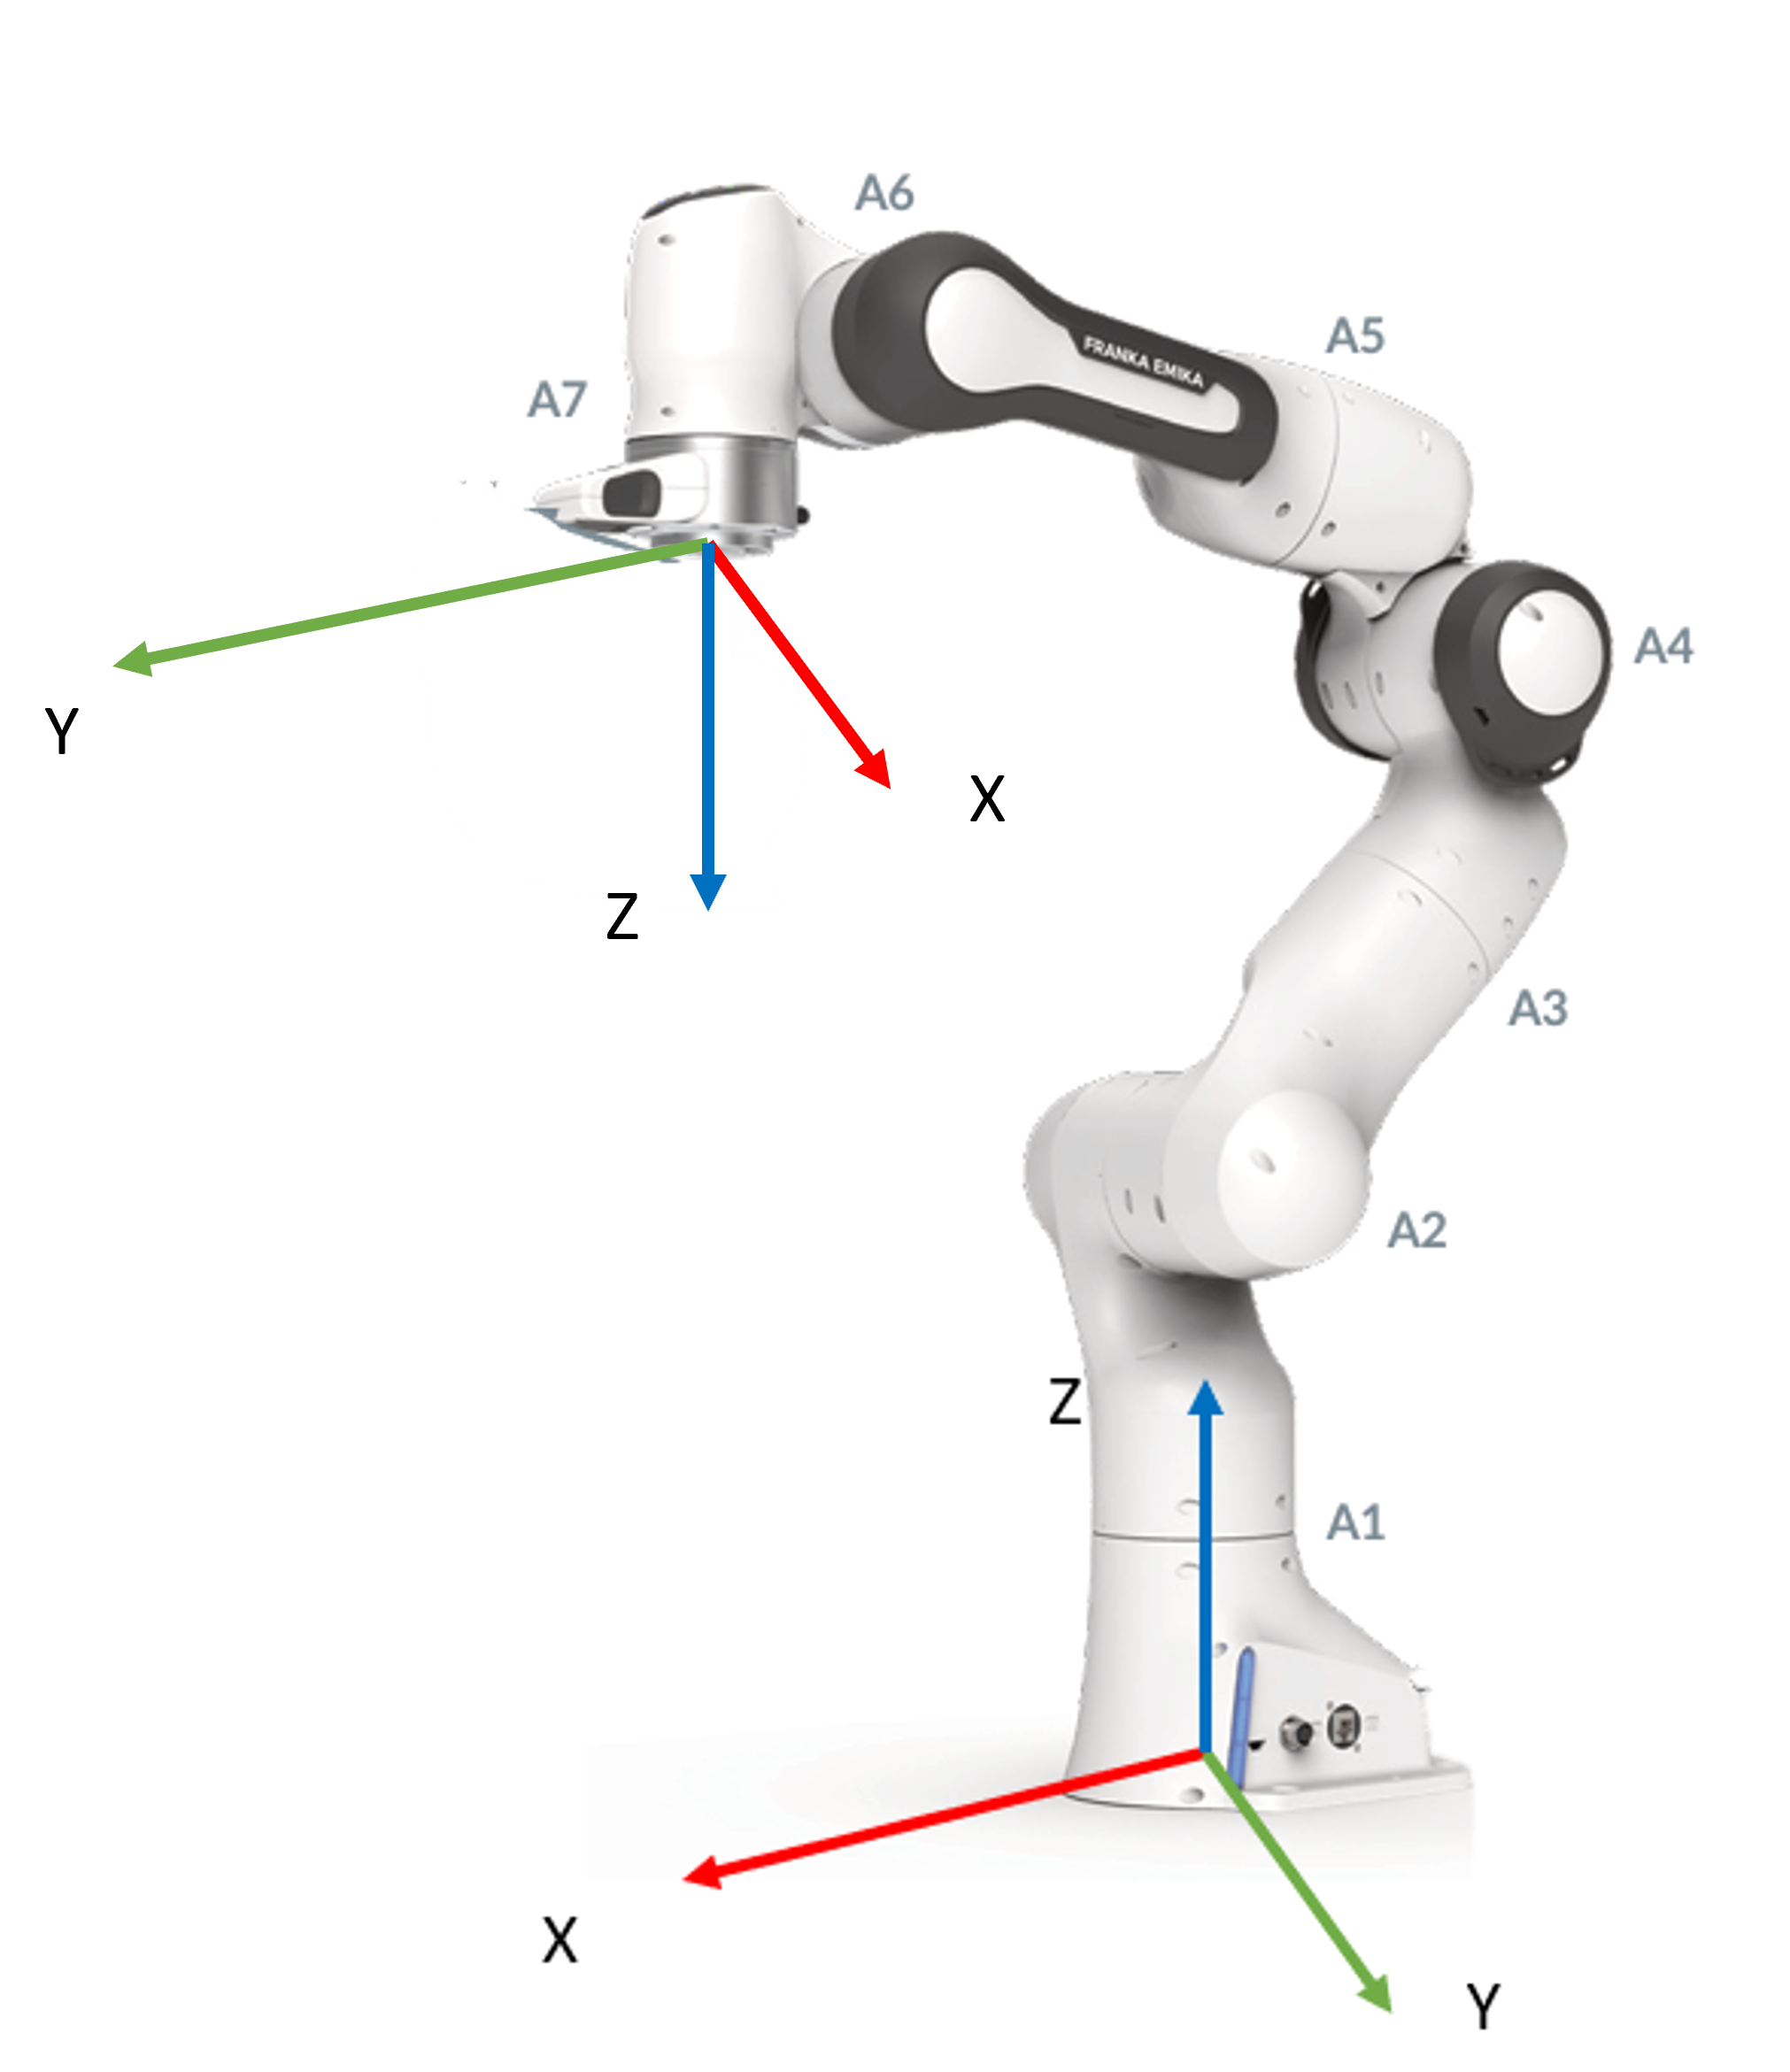
\includegraphics[scale=0.7]{pics/config2.png}
			\caption{The arms and joints of the Panda robot}
		\end{figure}
		
		Here are the dimensions of the robot.
		\begin{figure}[H]
			\begin{center}
				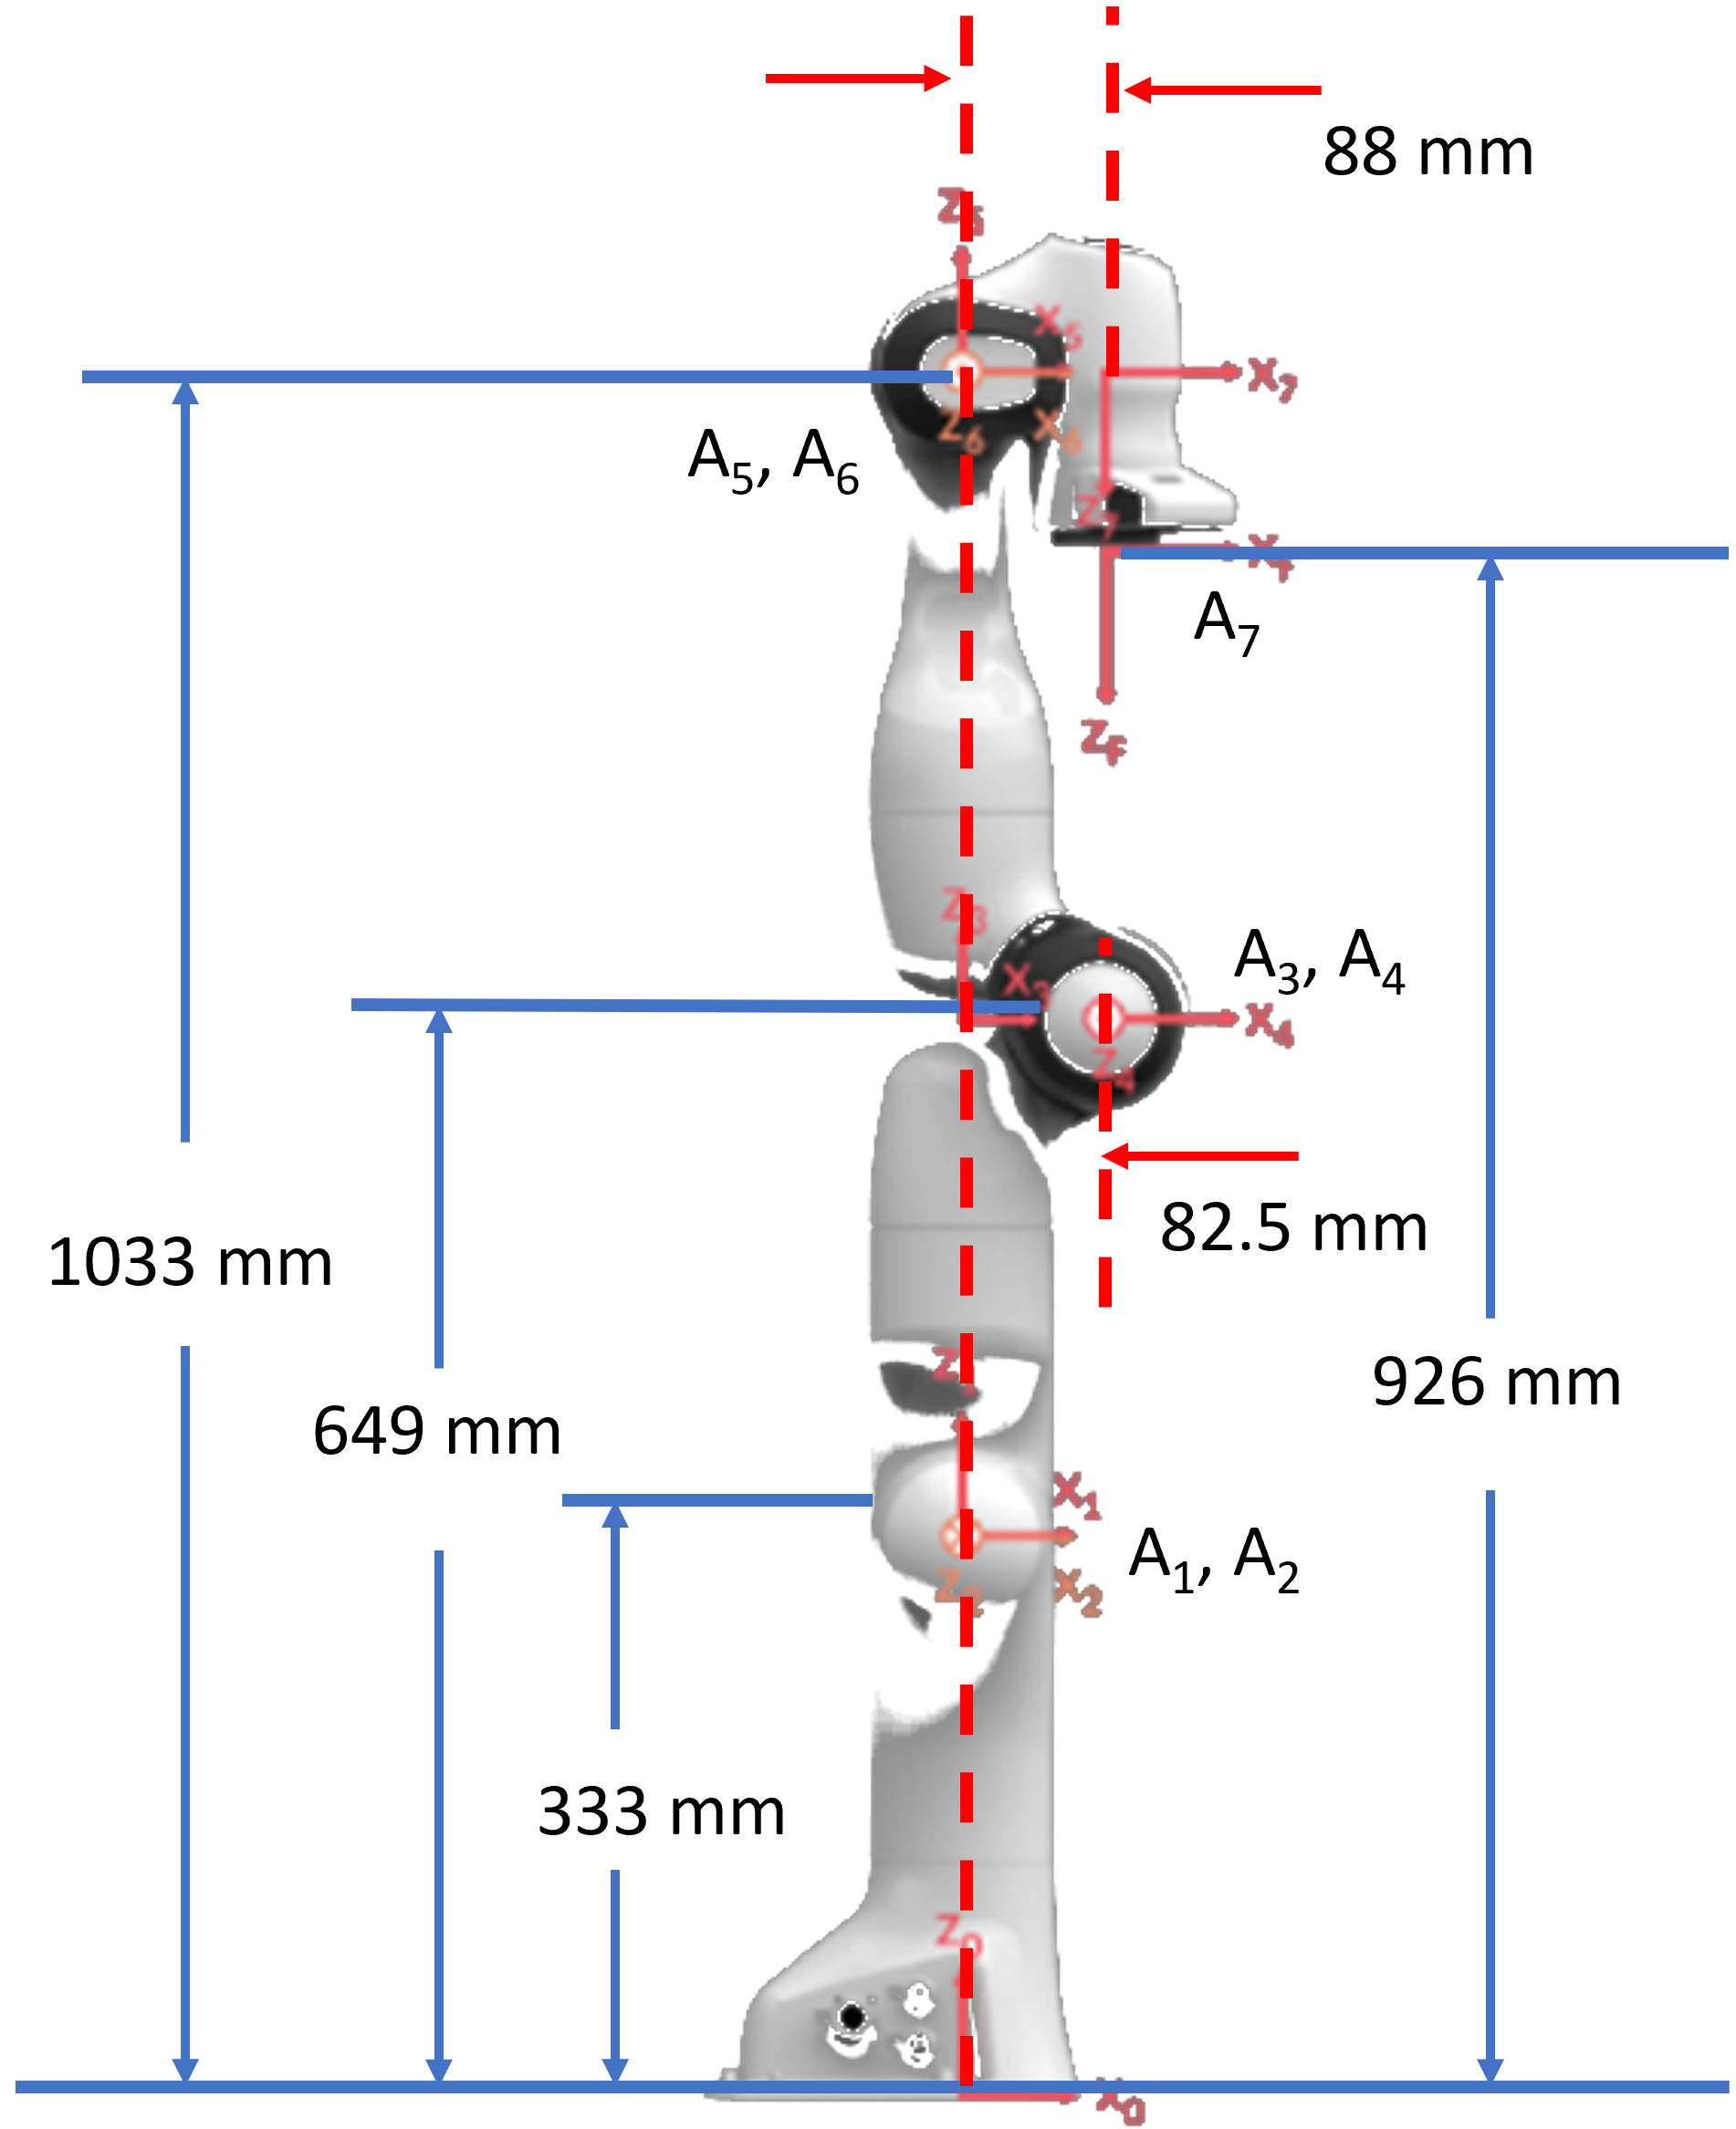
\includegraphics[scale=0.7]{pics/dims.png}
			\end{center}
			\caption{The parameters of Panda}
		\end{figure}
		
		The initial configuration of the end-effector is as follows:
		$$M = \begin{bmatrix}
			0.7071 & 0.7071 & 0 & 0.088\\
			0.7071 & -0.7071 & 0 & 0\\
			0 & 0 & -1 & 0.926 \\
			0 & 0 & 0 & 1 \\
		\end{bmatrix}$$
		
		But after attaching the cylindrical tool, the end-effector become the tip of the tool.
		\begin{figure}[H]
			\begin{center}
				\includegraphics[scale=0.7]{pics/robot-with-cylinder.png}
			\end{center}
			\caption{Panda with Cylindrical Tool}
		\end{figure}
		
		Therefore, the initial configuration of the cylindrical tool is
		\begin{equation}
			M = \begin{bmatrix}
				0.7071 & 0.7071 & 0 & 0.088\\
				0.7071 & -0.7071 & 0 & 0\\
				0 & 0 & -1 & 0.826 \\
				0 & 0 & 0 & 1 \\
			\end{bmatrix}
		\end{equation}
		
		Here are the twists for every joint.
		\begin{table}[H]
			\centering
			\caption{Normalized Twists}
			\begin{tabular}{|c|c|c|}
				\hline
				& $\omega_i$ & $v_i$ \\
				\hline
				A1 & $[0, 0, 1]^{T}$ & $[0, 0, 0]^{T}$ \\
				\hline
				A1 & $[0, 1, 0]^{T}$ & $[-0.333, 0, 0]^{T}$ \\
				\hline
				A3 & $[0, 0, 1]^{T}$ & $[0, 0, 0]^{T}$ \\
				\hline
				A4 & $[0, -1, 0]^{T}$ & $[0.649, 0, -0.0825]^{T}$ \\
				\hline
				A5 & $[0, 0, 1]^{T}$ & $[0, 0, 0]^{T}$ \\
				\hline
				A6 & $[0, -1, 0]^{T}$ & $[1.033, 0, 0]^{T}$ \\
				\hline
				A7 & $[0, 0, -1]^{T}$ & $[0, -0.088, 0]^{T}$ \\
				\hline
			\end{tabular}
		\end{table}
		Joint angle restrictions
		\begin{table}[H]
			\centering
			\caption{Joint Angle Limits}
			\begin{tabular}{|c|c|c|}
				\hline
				& min$/^\circ$& max$/^\circ$ \\
				\hline
				A1 & -166 & 166 \\
				\hline
				A1 & -101 & 101 \\
				\hline
				A3 & -166 & 166 \\
				\hline
				A4 & -176 & -4 \\
				\hline
				A5 & -166 & 166 \\
				\hline
				A6 & -1 & 215 \\
				\hline
				A7 & -166 & 166 \\
				\hline
			\end{tabular}
		\end{table}
		\section{Test Cases}
		\subsection*{2.0   Initial Guess}
		\begin{equation}
			q = \begin{bmatrix}
				0 & 0 & 0 & 0 & -\frac{\pi}{2} & 0 & \frac{\pi}{2} & 0
			\end{bmatrix}
		\end{equation}
		\begin{figure}[H]
			\includegraphics[width=\textwidth]{pics/init.png}
			\caption{Initial Configuration}
		\end{figure}
		And the axis of the tool is \((0, 0, -1)\). Therefore, when we want to minimize the change of the direction of the shaft, the axis of the tool at final configuration should also be \((0, 0, -1)\).
		\subsection{Forward Reach}
		\begin{equation}
			p_{goal} = \begin{bmatrix}
				0.75 &  0 & 0.3
			\end{bmatrix}
		\end{equation}
		\begin{figure}[H]
			\centering
			\includegraphics[width=0.8\textwidth]{pics/case1.png}
			\caption{Forward Reach}
		\end{figure}
		
		The equation of the virtual wall is 
		\begin{equation*}
			z = 0.29
		\end{equation*}
		
		\begin{figure}[H]
			\centering
			\includegraphics[width=\linewidth]{pics/ik_wall_test_1_5}
			\caption{Forward Reach with Wall}
		\end{figure}
		
		\subsection{Side Reach}
		\begin{equation}
			p_{goal} = \begin{bmatrix}
				0 & 0.5 & 0.3
			\end{bmatrix}
		\end{equation}
		\begin{figure}[H]
			\centering
			\includegraphics[width=0.7\linewidth]{pics/case2.png}
			\caption{Side Reach}
		\end{figure}
		
		The equation of the virtual wall is 
		\begin{equation*}
			x-z = -0.5
		\end{equation*}
		
		\begin{figure}[H]
			\centering
			\includegraphics[width=0.7\linewidth]{pics/ik_wall_test_2_8}
			\caption{Side Reach with Wall}
		\end{figure}
		
		\subsection{Backward Reach}
		\begin{equation}
			p_{goal} = \begin{bmatrix}
				-0.4 & 0.3 & 0.6
			\end{bmatrix}
		\end{equation}
		\begin{figure}[H]
			\centering
			\includegraphics[width=0.8\textwidth]{pics/case3.png}
			\caption{Backward Reach Configuration}
		\end{figure}
		
		The equation of the virtual wall is 
		\begin{equation*}
			\frac{1}{2}x + \frac{\sqrt{3}}{2}y = -0.1
		\end{equation*}
		
		\begin{figure}[H]
			\centering
			\includegraphics[width=0.8\linewidth]{pics/ik_wall_test_3_11}
			\caption{Backward Reach with Wall}
		\end{figure}
		\section{Programming Assignments a)}
		Implement an algorithm that moves the tool tip toward an arbitrary goal point while
		\begin{enumerate}\label{requirements1}
			\item Keeps tool tip as close as possible to $P_{\text{goal}}$ while never going beyond 3 mm from the goal
			\item and obeying joint limits.
		\end{enumerate}
		\subsection{Algorithm}
		This is the optimization-based control problem that need to solve \cite{Lynch_Park_2017}
		\begin{equation}
			\begin{aligned}
				\Delta \mathbf{q}_{\text{des}} &= \arg \min_{\Delta \mathbf{q}} \left\| \mathbf{D}(\Delta \mathbf{x}) \right\|^2 = \left\| \alpha \times \mathbf{t} + \epsilon + \mathbf{t} - \mathbf{p}_{\text{goal}} \right\|^2\\
				\alpha &= \mathbf{J}_{\alpha}(\mathbf{q}) \Delta \mathbf{q} \\
				\epsilon &= \mathbf{J}_{\epsilon}(\mathbf{q}) \Delta \mathbf{q} \\
				\| \alpha \times &\mathbf{t} + \epsilon + \mathbf{t} - \mathbf{p}_{\text{goal}} \| \leq 3 \\
				\mathbf{q}_L - \mathbf{q} &\leq \Delta \mathbf{q} \leq \mathbf{q}_U - \mathbf{q}
			\end{aligned}
		\end{equation}
		
		This algorithms is implemented in \texttt{opti\_ik\_space.m}
		\begin{algorithm}[H]
			\caption{\texttt{opti\_ik\_space} Optimization-based Inverse Kinematics Algorithm in Space Frame}
			\begin{algorithmic}[1]
				\State \textbf{Inputs:} $M$ (Initial Configuration), $S$ (Normalized Twists), $p_{\text{goal}}$ (Destination), $q_{\text{init}}$ (Initial Guess), $qL$ (Joint Lower Limits), $qU$ (Joint Upper Limits)
				\State \textbf{Initialize:} Set $q \gets q_{\text{init}}$, $\epsilon \gets 0.003$, $\text{error} \gets 1$.
				\While{$\text{error} > \epsilon$}
				\State Compute forward kinematics: $T_{\text{sb}} \gets \text{FK\_space}(M, S, q)$.
				\State Extract current position: $t \gets T_{\text{sb}}(1:3, 4)$.
				\State Compute position error: $\text{error} \gets \| t - p_{\text{des}} \|$.
				\State Compute space Jacobian: $J \gets \text{J\_space}(S, q)$.
				\State Extract submatrices: $J_{\alpha} \gets J(1:3, :)$, $J_p \gets J(4:6, :)$.
				\State Compute coefficient matrix: $A \gets J_p - \text{vecToso3}(t) \cdot J_{\alpha}$.
				\State Compute residual: $b \gets p_{\text{des}} - t$.
				\State Compute bounds: $\text{lb} \gets qL - q$, $\text{ub} \gets qU - q$.
				\State Solve constrained least-squares problem: $\Delta q \gets \text{lsqlin}(A, b, \text{lb}, \text{ub})$.
				\State Update joint angles: $q \gets q + \Delta q$.
				\EndWhile
				\State \textbf{Return:} $q$.
			\end{algorithmic}
		\end{algorithm}
		Note that: \begin{enumerate}
			\item The calculation of forward kinematics and Jacobian matrix are in space frame.
			\item We used the \texttt{lsqlin} function in MATLAB to implement the optimization process.
			\item Requirement \(\| \alpha \times \mathbf{t} + \epsilon + \mathbf{t} - \mathbf{p}_{\text{goal}} \| \leq 3\) is fulfilled implicitly in this program by setting the threshold to be small enough (Here we set it to be 0.003 or 3 mm).
		\end{enumerate}
		
		\subsection{Test}
		\subsubsection{Case 1: Forward Reach}
		In this case, five iterations are needed to reach the target
		\begin{figure}[H]
			\begin{minipage}{0.33\textwidth}
				\centering
				\includegraphics[width=\textwidth]{pics/ik_space_test_1_0.png}
				\caption{Initial Configuration}
			\end{minipage}
			\begin{minipage}{0.33\textwidth}
				\centering
				\includegraphics[width=\textwidth]{pics/ik_space_test_1_1.png}
				\caption{Iteration 1}
			\end{minipage}
			\begin{minipage}{0.33\textwidth}
				\centering
				\includegraphics[width=\textwidth]{pics/ik_space_test_1_2.png}
				\caption{Iteration 2}
			\end{minipage}
		\end{figure}
		\begin{figure}[H]
			\begin{minipage}{0.33\textwidth}
				\centering
				\includegraphics[width=\textwidth]{pics/ik_space_test_1_3.png}
				\caption{Iteration 3}
			\end{minipage}
			\begin{minipage}{0.33\textwidth}
				\centering
				\includegraphics[width=\textwidth]{pics/ik_space_test_1_4.png}
				\caption{Iteration 4}
			\end{minipage}
			\begin{minipage}{0.33\textwidth}
				\centering
				\includegraphics[width=\textwidth]{pics/ik_space_test_1_5.png}
				\caption{Iteration 5}
			\end{minipage}
		\end{figure}
		The final position of the tool tip is \((0.750, 0, 0.300)\). And the final direction of the tool axis is \((0.262, 0.000, -0.965)\)
		\subsubsection{Case 2: Side Reach}
		Here we omit the iteration process, just give the final result. Ten iterations are need to converge. The final position of the tool tip is \((0.000, 0.500, 0.300)\). And the final direction of the tool axis is \((-0.395, -0.398, -0.828)\)
		\begin{figure}[H]
			\includegraphics{pics/ik_space_test_2_10}
			\caption{Final Configuration in the Side Reach Case}
		\end{figure}
		\subsubsection{Case 3: Backward Reach}
		14 Iterations are needed to converge. The final position of the tool tip is \((-0.400, 0.300, 0.600)\). And the final direction of the tool axis is \((-0.068, 0.038, -0.997)\)
		\begin{figure}[H]
			\centering
			\includegraphics[width=0.8\textwidth]{pics/ik_space_test_3_7}
			\caption{Final Configuration in the Backward Reach Case}
		\end{figure}
		\section{Programming Assignments b)}
		Similar to a), implement an algorithm that moves the tool tip toward an arbitrary goal point while
		\begin{enumerate}
			\item Keeps tool tip as close as possible to $P_{\text{goal}}$ while never going beyond 3 mm from the goal
			\item Obeying joint limits.
			\item Minimizes the change in direction of the tool shaft during motion
		\end{enumerate}
		\subsection{Algorithm}
		This is the optimization-based control problem that to be solved
		\begin{equation}
			\begin{aligned}
				\Delta \mathbf{q}_{\text{des}} &= \arg \min_{\Delta \mathbf{q}} \left\| \mathbf{D}(\Delta \mathbf{x}) \right\|^2 = \left\| \alpha \times \mathbf{t} + \epsilon + \mathbf{t} - \mathbf{p}_{\text{goal}} \right\|^2 + \eta \|\alpha \times \mathbf{R} \cdot \mathbf{z}\|^2\\
				\alpha &= \mathbf{J}_{\alpha}(\mathbf{q}) \Delta \mathbf{q} \\
				\epsilon &= \mathbf{J}_{\epsilon}(\mathbf{q}) \Delta \mathbf{q} \\
				\| \alpha \times &\mathbf{t} + \epsilon + \mathbf{t} - \mathbf{p}_{\text{goal}} \| \leq 3 \\
				\mathbf{q}_L - \mathbf{q} &\leq \Delta \mathbf{q} \leq \mathbf{q}_U - \mathbf{q}
			\end{aligned}
		\end{equation}
		
		This algorithms is implemented in \texttt{opti\_ik\_angle\_space.m}
		\begin{algorithm}[H]
			\caption{\texttt{opti\_ik\_angle\_space} Optimization-based Inverse Kinematics Algorithm while Minimizing Axis Angle Change in Space Frame}
			\begin{algorithmic}[1]
				\Function{opti\_ik\_angle\_space}{$\mathbf{M}, \mathbf{S}, \mathbf{p}_{\text{goal}}, \mathbf{q}_{\text{init}}, \mathbf{q}_L, \mathbf{q}_U$}
				\State \textbf{Inputs:} $M$ (Initial Configuration), $S$ (Normalized Twists), $p_{\text{goal}}$ (Destination), $q_{\text{init}}$ (Initial Guess), $qL$ (Joint Lower Limits), $qU$ (Joint Upper Limits)
				\State Set constants: \( \epsilon_1 = 0.003 \), \( \epsilon_2 = 0.01 \), \( \eta = 0.1 \), \( \mathbf{z}_s = [0, 0, 1]^T \).
				\State Initialize: \( \mathbf{q} = \mathbf{q}_{\text{init}} \).
				\State Initialize errors: \( \text{error}_1 = 1 \), \( \text{error}_2 = 1 \).
				\While{\( \text{error}_1 > \epsilon_1 \text{ or } \text{error}_2 > \epsilon_2 \)}
				\State Compute forward kinematics: \( \mathbf{T}_{sb} = \text{FK\_space}(\mathbf{M}, \mathbf{S}, \mathbf{q}) \).
				\State Extract current orientation: \( \mathbf{R}_z = \mathbf{T}_{sb}(1:3, 1:3) \cdot \mathbf{z}_s \).
				\State Extract current position: \( \mathbf{t} = \mathbf{T}_{sb}(1:3, 4) \).
				\State Compute errors:
				\State \quad \( \text{error}_1 = \|\mathbf{t} - \mathbf{p}_{\text{goal}}\| \).
				\State \quad \( \text{error}_2 = \|\mathbf{R}_z - \mathbf{R}_{\text{init}}\| \).
				\State Compute space Jacobian: \( \mathbf{J} = \text{J\_space}(\mathbf{S}, \mathbf{q}) \).
				\State Extract sub-Jacobians: \( \mathbf{J}_\alpha = \mathbf{J}(1:3, :), \mathbf{J}_p = \mathbf{J}(4:6, :) \).
				\State Formulate least-squares system:
				\State \quad \( \mathbf{A}_1 = \mathbf{J}_p - \text{vecToso3}(\mathbf{t}) \cdot \mathbf{J}_\alpha \).
				\State \quad \( \mathbf{b}_1 = \mathbf{p}_{\text{goal}} - \mathbf{t} \).
				\State \quad \( \mathbf{A}_2 = \sqrt{\eta} \cdot \text{vecToso3}(\mathbf{R}_z) \cdot \mathbf{J}_\alpha \).
				\State \quad \( \mathbf{b}_2 = -\sqrt{\eta} \cdot (\mathbf{R}_{\text{init}} - \mathbf{R}_z) \).
				\State Define joint bounds: \( \mathbf{lb} = \mathbf{q}_L - \mathbf{q} \), \( \mathbf{ub} = \mathbf{q}_U - \mathbf{q} \).
				\State Solve constrained least-squares: \( \Delta \mathbf{q}_{\text{dir}} = \text{lsqlin}([\mathbf{A}_1; \mathbf{A}_2], [\mathbf{b}_1; \mathbf{b}_2], [], [], [], [], \mathbf{lb}, \mathbf{ub}) \).
				\State Line search to get best step length $\alpha$
				\For{\(i = 1\) to \(\text{max\_iter}\)}
				\State Compute \(q_{\text{candidate}} \gets q + \alpha \cdot \delta q_{\text{dir}}\)
				\State Compute \(T_{\text{sb}}^{\text{candidate}} \gets \text{FK\_space}(M, S, q_{\text{candidate}})\)
				\State Extract \(t_{\text{candidate}} \gets T_{\text{sb}}^{\text{candidate}}(1:3, 4)\)
				\If{\(\|t_{\text{candidate}} - p_{\text{goal}}\|_2 > \|t - p_{\text{goal}}\|_2\)}
				\State Update \(\alpha \gets \alpha \cdot \beta\), where \(\beta \in (0, 1)\)
				\State Continue
				\EndIf
				\EndFor
				\State Update joint angles: \( \mathbf{q} = \mathbf{q} + \alpha \Delta \mathbf{q} \).
				\EndWhile
				\State \Return \( \mathbf{q} \)
				\EndFunction
			\end{algorithmic}
		\end{algorithm}
		Note that: \begin{enumerate}
			\item The calculation of forward kinematics and Jacobian matrix are in space frame.
			\item There are two weights, one for the distance to the target and one for the change in direction of the tool axis. But since this is an parameter optimization problem. What really matters is relative weight. Therefore, we just use one weight \(\eta\) (which is set to be 0.1) for the change in direction of the tool axis.
			\item We used the \texttt{lsqlin} function in MATLAB to implement the optimization process.
			\item Requirement \(\| \alpha \times \mathbf{t} + \epsilon + \mathbf{t} - \mathbf{p}_{\text{goal}} \| \leq 3\) is fulfilled implicitly in this program by setting the threshold to be small enough.
			\item We used two criterion (the distance to target and axis change) the judge the convergence.
			\item We used line search method to get appropriate step length $\alpha$. This could improve the program's robustness, because of the linearization and small angle approximation of the method \cite{nocedal2006numerical}. 
		\end{enumerate}
		\subsection{Test}
		\subsubsection{Case 1: Forward Reach}
		In this case, five iterations are needed to reach the target
		\begin{figure}[H]
			\begin{minipage}{0.33\textwidth}
				\centering
				\includegraphics[width=\textwidth]{pics/ik_angle_space_test_1_0.png}
				\caption{Initial Configuration}
			\end{minipage}
			\begin{minipage}{0.33\textwidth}
				\centering
				\includegraphics[width=\textwidth]{pics/ik_angle_space_test_1_1.png}
				\caption{Iteration 1}
			\end{minipage}
			\begin{minipage}{0.33\textwidth}
				\centering
				\includegraphics[width=\textwidth]{pics/ik_angle_space_test_1_2.png}
				\caption{Iteration 2}
			\end{minipage}
		\end{figure}
		\begin{figure}[H]
			\begin{minipage}{0.33\textwidth}
				\centering
				\includegraphics[width=\textwidth]{pics/ik_angle_space_test_1_3.png}
				\caption{Iteration 3}
			\end{minipage}
			\begin{minipage}{0.33\textwidth}
				\centering
				\includegraphics[width=\textwidth]{pics/ik_angle_space_test_1_4.png}
				\caption{Iteration 4}
			\end{minipage}
			\begin{minipage}{0.33\textwidth}
				\centering
				\includegraphics[width=\textwidth]{pics/ik_angle_space_test_1_5.png}
				\caption{Iteration 5}
			\end{minipage}
		\end{figure}
		The final position of the tool tip is \((0.750, 0.000, 0.300)\). And the final direction of the tool axis is \((-0.00, -0.000, -1.00)\).
		\subsubsection{Case 2: Side Reach}
		8 Iterations are need to converge. The final position of the tool tip is \((0.000, 0.500, 0.300)\). And the final direction of the tool axis is \((-0.000, -0.000, -1.000)\)
		\begin{figure}[H]
			\centering
			\includegraphics{pics/ik_angle_space_test_2_8}
			\caption{Final Configuration in the Side Reach Case}
		\end{figure}
		\subsubsection{Case 3: Backward Reach}
		8 Iterations are need to converge. The final position of the tool tip is \((-0.400, 0.300, 0.600)\). And the final direction of the tool axis is \((-0.000, 0.000, -1.000)\)
		\begin{figure}[H]
			\centering
			\includegraphics[width=0.8\textwidth]{pics/ik_angle_space_test_3_6}
			\caption{Final Configuration in the Backward Reach Case}
		\end{figure}
		\section{Programming Assignments c)}
		Repeat part (a) and (b) while having a \textbf{virtual wall} defined close to the desired goal point.
		\subsection{Algorithm}
		This is the optimization-based control problem that need to be solved with a virtual wall but without minimizing the change of tool shaft.
		\begin{equation}\label{noaxis}
			\begin{aligned}
				\Delta \mathbf{q}_{\text{des}} &= \arg \min_{\Delta \mathbf{q}} \left\| \mathbf{D}(\Delta \mathbf{x}) \right\|^2 = \left\| \alpha \times \mathbf{t} + \epsilon + \mathbf{t} - \mathbf{p}_{\text{goal}} \right\|^2\\
				\alpha &= \mathbf{J}_{\alpha}(\mathbf{q}) \Delta \mathbf{q} \\
				\epsilon &= \mathbf{J}_{\epsilon}(\mathbf{q}) \Delta \mathbf{q} \\
				\mathbf{n}_{\text{wall}} & \cdot( \alpha \times \mathbf{t} + \epsilon + \mathbf{t} - \mathbf{p}_{\text{wall}}) \ge 0 \\
				\| \alpha \times &\mathbf{t} + \epsilon + \mathbf{t} - \mathbf{p}_{\text{goal}} \| \leq 3 \\
				\mathbf{q}_L - \mathbf{q} &\leq \Delta \mathbf{q} \leq \mathbf{q}_U - \mathbf{q}
			\end{aligned}
		\end{equation}
		
		And this is the optimization-based control problem with a virtual wall while minimizing the change of tool shaft.
		\begin{equation}\label{withaxis}
			\begin{aligned}
				\Delta \mathbf{q}_{\text{des}} &= \arg \min_{\Delta \mathbf{q}} \left\| \mathbf{D}(\Delta \mathbf{x}) \right\|^2 = \left\| \alpha \times \mathbf{t} + \epsilon + \mathbf{t} - \mathbf{p}_{\text{goal}} \right\|^2 + \eta \|\alpha \times \mathbf{R} \cdot \mathbf{z}\|^2\\
				\alpha &= \mathbf{J}_{\alpha}(\mathbf{q}) \Delta \mathbf{q} \\
				\epsilon &= \mathbf{J}_{\epsilon}(\mathbf{q}) \Delta \mathbf{q} \\
				\mathbf{n}_{\text{wall}} & \cdot( \alpha \times \mathbf{t} + \epsilon + \mathbf{t} - \mathbf{p}_{\text{wall}}) \ge 0 \\
				\| \alpha \times &\mathbf{t} + \epsilon + \mathbf{t} - \mathbf{p}_{\text{goal}} \| \leq 3 \\
				\mathbf{q}_L - \mathbf{q} &\leq \Delta \mathbf{q} \leq \mathbf{q}_U - \mathbf{q}
			\end{aligned}
		\end{equation}
		where \(\mathbf{n}_{\text{wall}}\) is the normal vector of the virtual wall, while \(\mathbf{p}_{\text{goal}}\) is a point on the virtual wall.
		
		The above two algorithms only differs from their corresponding part (a) and part (b) in adding an additional inequality constraint. So, we omit their algorithms here.
		\subsection{Test of \ref{noaxis} without Minimizing the Change in Direction of the Tool Shaft}
		\subsubsection{Case 1: Forward Reach}
		In this case, five iterations are needed to reach the target
		\begin{figure}[H]
			\begin{minipage}{0.33\textwidth}
				\centering
				\includegraphics[width=\textwidth]{pics/ik_wall_test_1_0.png}
				\caption{Initial Configuration}
			\end{minipage}
			\begin{minipage}{0.33\textwidth}
				\centering
				\includegraphics[width=\textwidth]{pics/ik_wall_test_1_1.png}
				\caption{Iteration 1}
			\end{minipage}
			\begin{minipage}{0.33\textwidth}
				\centering
				\includegraphics[width=\textwidth]{pics/ik_wall_test_1_2.png}
				\caption{Iteration 2}
			\end{minipage}
		\end{figure}
		\begin{figure}[H]
			\begin{minipage}{0.33\textwidth}
				\centering
				\includegraphics[width=\textwidth]{pics/ik_wall_test_1_3.png}
				\caption{Iteration 3}
			\end{minipage}
			\begin{minipage}{0.33\textwidth}
				\centering
				\includegraphics[width=\textwidth]{pics/ik_wall_test_1_4.png}
				\caption{Iteration 4}
			\end{minipage}
			\begin{minipage}{0.33\textwidth}
				\centering
				\includegraphics[width=\textwidth]{pics/ik_wall_test_1_5.png}
				\caption{Iteration 5}
			\end{minipage}
		\end{figure}
		
		The final position of the tool tip is \((0.750, 0.000, 0.300)\). And the final direction of the tool axis is \((0.287, -0.000, -0.958)\).
		\subsubsection{Case 2: Side Reach}
		
		8 iterations are needed to reach convergence.
		The final position of the tool tip is \((0.000, 0.500, 0.300)\). And the final direction of the tool axis is \((-0.452, -0.345, -0.823)\)
		\begin{figure}[H]
			\centering
			\includegraphics[width=0.7\textwidth]{pics/ik_wall_test_2_8}
			\caption{Final Configuration in the Side Reach Case}
		\end{figure}
		\subsubsection{Case 3: Backward Reach}
		11 iterations are needed to reach convergence.
		The final position of the tool tip is \((-0.400, 0.300, 0.600)\). And the final direction of the tool axis is \((-0.129, -0.0155, -0.991)\)
		\begin{figure}[H]
			\includegraphics[width=0.8\textwidth]{pics/ik_wall_test_3_11}
			\caption{Final Configuration in the Backward Reach Case}
		\end{figure}
		
		\subsection{Test of \ref{withaxis} while Minimizing the Change in Direction of the Tool Shaft}
		\subsubsection{Case 1: Forward Reach}
		In this case, six iterations are needed to reach the target (first five iterations are plotted here)
		\begin{figure}[H]
			\begin{minipage}{0.33\textwidth}
				\centering
				\includegraphics[width=\textwidth]{pics/ik_angle_wall_test_1_0.png}
				\caption{Initial Configuration}
			\end{minipage}
			\begin{minipage}{0.33\textwidth}
				\centering
				\includegraphics[width=\textwidth]{pics/ik_angle_wall_test_1_1.png}
				\caption{Iteration 1}
			\end{minipage}
			\begin{minipage}{0.33\textwidth}
				\centering
				\includegraphics[width=\textwidth]{pics/ik_angle_wall_test_1_2.png}
				\caption{Iteration 2}
			\end{minipage}
		\end{figure}
		\begin{figure}[H]
			\begin{minipage}{0.33\textwidth}
				\centering
				\includegraphics[width=\textwidth]{pics/ik_angle_wall_test_1_3.png}
				\caption{Iteration 3}
			\end{minipage}
			\begin{minipage}{0.33\textwidth}
				\centering
				\includegraphics[width=\textwidth]{pics/ik_angle_wall_test_1_4.png}
				\caption{Iteration 4}
			\end{minipage}
			\begin{minipage}{0.33\textwidth}
				\centering
				\includegraphics[width=\textwidth]{pics/ik_angle_wall_test_1_5.png}
				\caption{Iteration 5}
			\end{minipage}
		\end{figure}
		
		\subsubsection{Case 2: Side Reach}
		7 iterations are needed to reach convergence.
		The final position of the tool tip is \((0.000, 0.500, 0.300)\). And the final direction of the tool axis is \((-0.000, -0.000, -1.000)\)
		\begin{figure}[H]
			\centering
			\includegraphics[width=0.8\textwidth]{pics/ik_angle_wall_test_2_7}
			\caption{Final Configuration in the Side Reach Case}
		\end{figure}
		\subsubsection{Case 3: Backward Reach}
		10 iterations are needed to reach convergence.
		The final position of the tool tip is \((-0.400, 0.300, 0.600)\). And the final direction of the tool axis is \((-0.000, -0.000, -1.000)\)
		\begin{figure}[H]
			\centering
			\includegraphics[width=0.8\textwidth]{pics/ik_angle_wall_test_3_10}
			\caption{Final Configuration in the Backward Reach Case}
		\end{figure}
		
		\section{Comparison}
		The comparison is implemented in \texttt{compare.m}. For the visualization, we separately created corresponding files \texttt{xxx\_visualize.m} for all the four algorithms mentioned earlier, which basically completed the same task as their original version but output additional three variables: distance to the goal, change of tool shaft direction, and distance to the wall.
		
		And we adopt the following notations:
		\begin{table}[H]
			\caption{Notations}
			\begin{tabular}{|c|c|}
				\hline
				notation & meaning \\
				\hline
				ik & approximating a point in part (a) \\
				\hline
				angle & approximating a point while minimizing axis angle change in part (b) \\
				\hline
				wall & approximating a point with a wall in part (c) \\
				\hline
				angle\_wall & approximating a point with a wall while minimizing axis angle change in part (c) \\
				\hline
			\end{tabular}
		\end{table}
		
		\subsection{Case 1: Forward Reach}
		\begin{figure}[H]
			\centering
			\includegraphics[width=\textwidth]{pics/ik_methods_comparison_1}
			\caption{Comparison of Methods in the Forward Reach Case}
		\end{figure}
		\subsubsection{Case 2: Side Reach}
		\begin{figure}[H]
			\centering
			\includegraphics[width=\textwidth]{pics/ik_methods_comparison_2}
			\caption{Final Configuration in the Side Reach Case}
		\end{figure}
		\subsubsection{Case 3: Backward Reach}
		\begin{figure}[H]
			\centering
			\includegraphics[width=\textwidth]{pics/ik_methods_comparison_3}
			\caption{Comparison of Methods in the Backward Reach Case}
		\end{figure}
		\section{Summary}
		\begin{enumerate}
			\item All the four methods successfully reached the goal points in all the three cases (shown in the upper subplots).
			\item For the three cases, the third case (Backward Reach) requires the most number of iterations because it is the hardest to reach.
			\item Of all the four methods, the vanilla inverse kinematics method (denoted by "ik") requires the most number of iterations because it does use line search method. Since we are using Jacobian matrix and small angle rotation transformation which are only applicable for small joint angle change, it is not doing well for large transformation, especially for side reach and backward reach cases.
			\item The methods involving minimizing the change of tool axis direction (denoted by "angle" and "angle\_wall") successfully reached their mission, reaching 0 in the change of tool shaft (or orientation error shown in the middle subplots).
			\item The methods virtual wall constraints successfully kept the distance to the wall greater than 0 (shown in the lower subplots).
		\end{enumerate}
		
    \printbibliography
\end{document}